\graphicspath{{intro/}{theory/}}

% Header
\renewcommand\evenpagerightmark{{\scshape\small Chapter 2}}
\renewcommand\oddpageleftmark{{\scshape\small Dark Matter Scenarios Beyond the Standard Model}}

%\renewcommand{\bibname}{References}

\hyphenation{}

\chapter{Dark Matter Scenarios Beyond the Standard Model}
\label{ch:theory}

In modern particle physics, the fundamental structure of matter at subatomic scales is described by the Standard Model~\cite{Peskin:257493, BSMWiley}, which has already predicted many experimental results and is today considered among the most thoroughly tested scientific theories. The Higgs boson, the last missing piece which was predicted more than 50 years ago, was recently discovered at the \ac{LHC} in 2012~\cite{Aad:2012tfa, Chatrchyan:2012xdj}, thus completing this elegant theory. Although it has survived many precision tests so far, the Standard Model only describes 5\% of the matter and energy in the known universe and is unable to explain many unresolved questions and observations, such as the baryon asymmetry, dark matter and dark energy, the neutrino masses, the incorporation of gravity, and the hierarchy problem.

In this chapter, a brief description of the Standard Model is first given in Section~\ref{sec:SM}, including its shortcomings. In Section~\ref{sec:DM}, one of the missing pieces in the Standard Model, dark matter, is discussed. The observational evidence for dark matter, as well as possible models and detection mechanisms are detailed. Finally, in Section~\ref{sec:SIMP} one of the dark matter models considered in this thesis is described in detail.

\section{The Standard Model of Particle Physics}
\label{sec:SM}

The Standard Model of elementary particle physics has been developed during the second half of the 20th century, and reached its current formulation in the 1970's with the combination of the electromagnetic and weak interactions into the electroweak interaction~\cite{Glashow:1959wxa, Weinberg:1967tq, Salam:1959zz}, incorporating the Brout-Englert-Higgs (BEH) mechanism~\cite{Englert:1964et,Higgs:1964pj,Guralnik:1964eu}, and the addition of asymptotic freedom~\cite{Gross:1973id, Politzer:1973fx} into the theory of the strong interaction.
% , which describes how particles obtain their mass. 
It is a quantum field theory which describes the fundamental particles and their interactions, incorporating three of the four fundamental forces. While this consistent framework describes the electromagnetic force and the weak and strong interactions, the fourth interaction, gravity, has not yet been included successfully.

\subsection{Elementary particles and their interactions}

All ordinary matter we see around us is built up from atoms, which consist of negatively charged electrons and a positively charged atomic nucleus, formed by protons and neutrons, which in turn consist of up and down quarks. The electrons and the up and down quarks are fundamental particles called fermions. Although all ordinary matter can be built from this so-called first generation of fermions, there are twelve fermions with different flavours in total, six quarks and six leptons, grouped in three generations with increasing mass, as shown in Figure~\ref{fig:SM}. The electrically neutral neutrinos interact only via the weak interaction, which complicates their observation, but they can be detected in dedicated experiments.

\begin{figure}[ht]
  \centering
  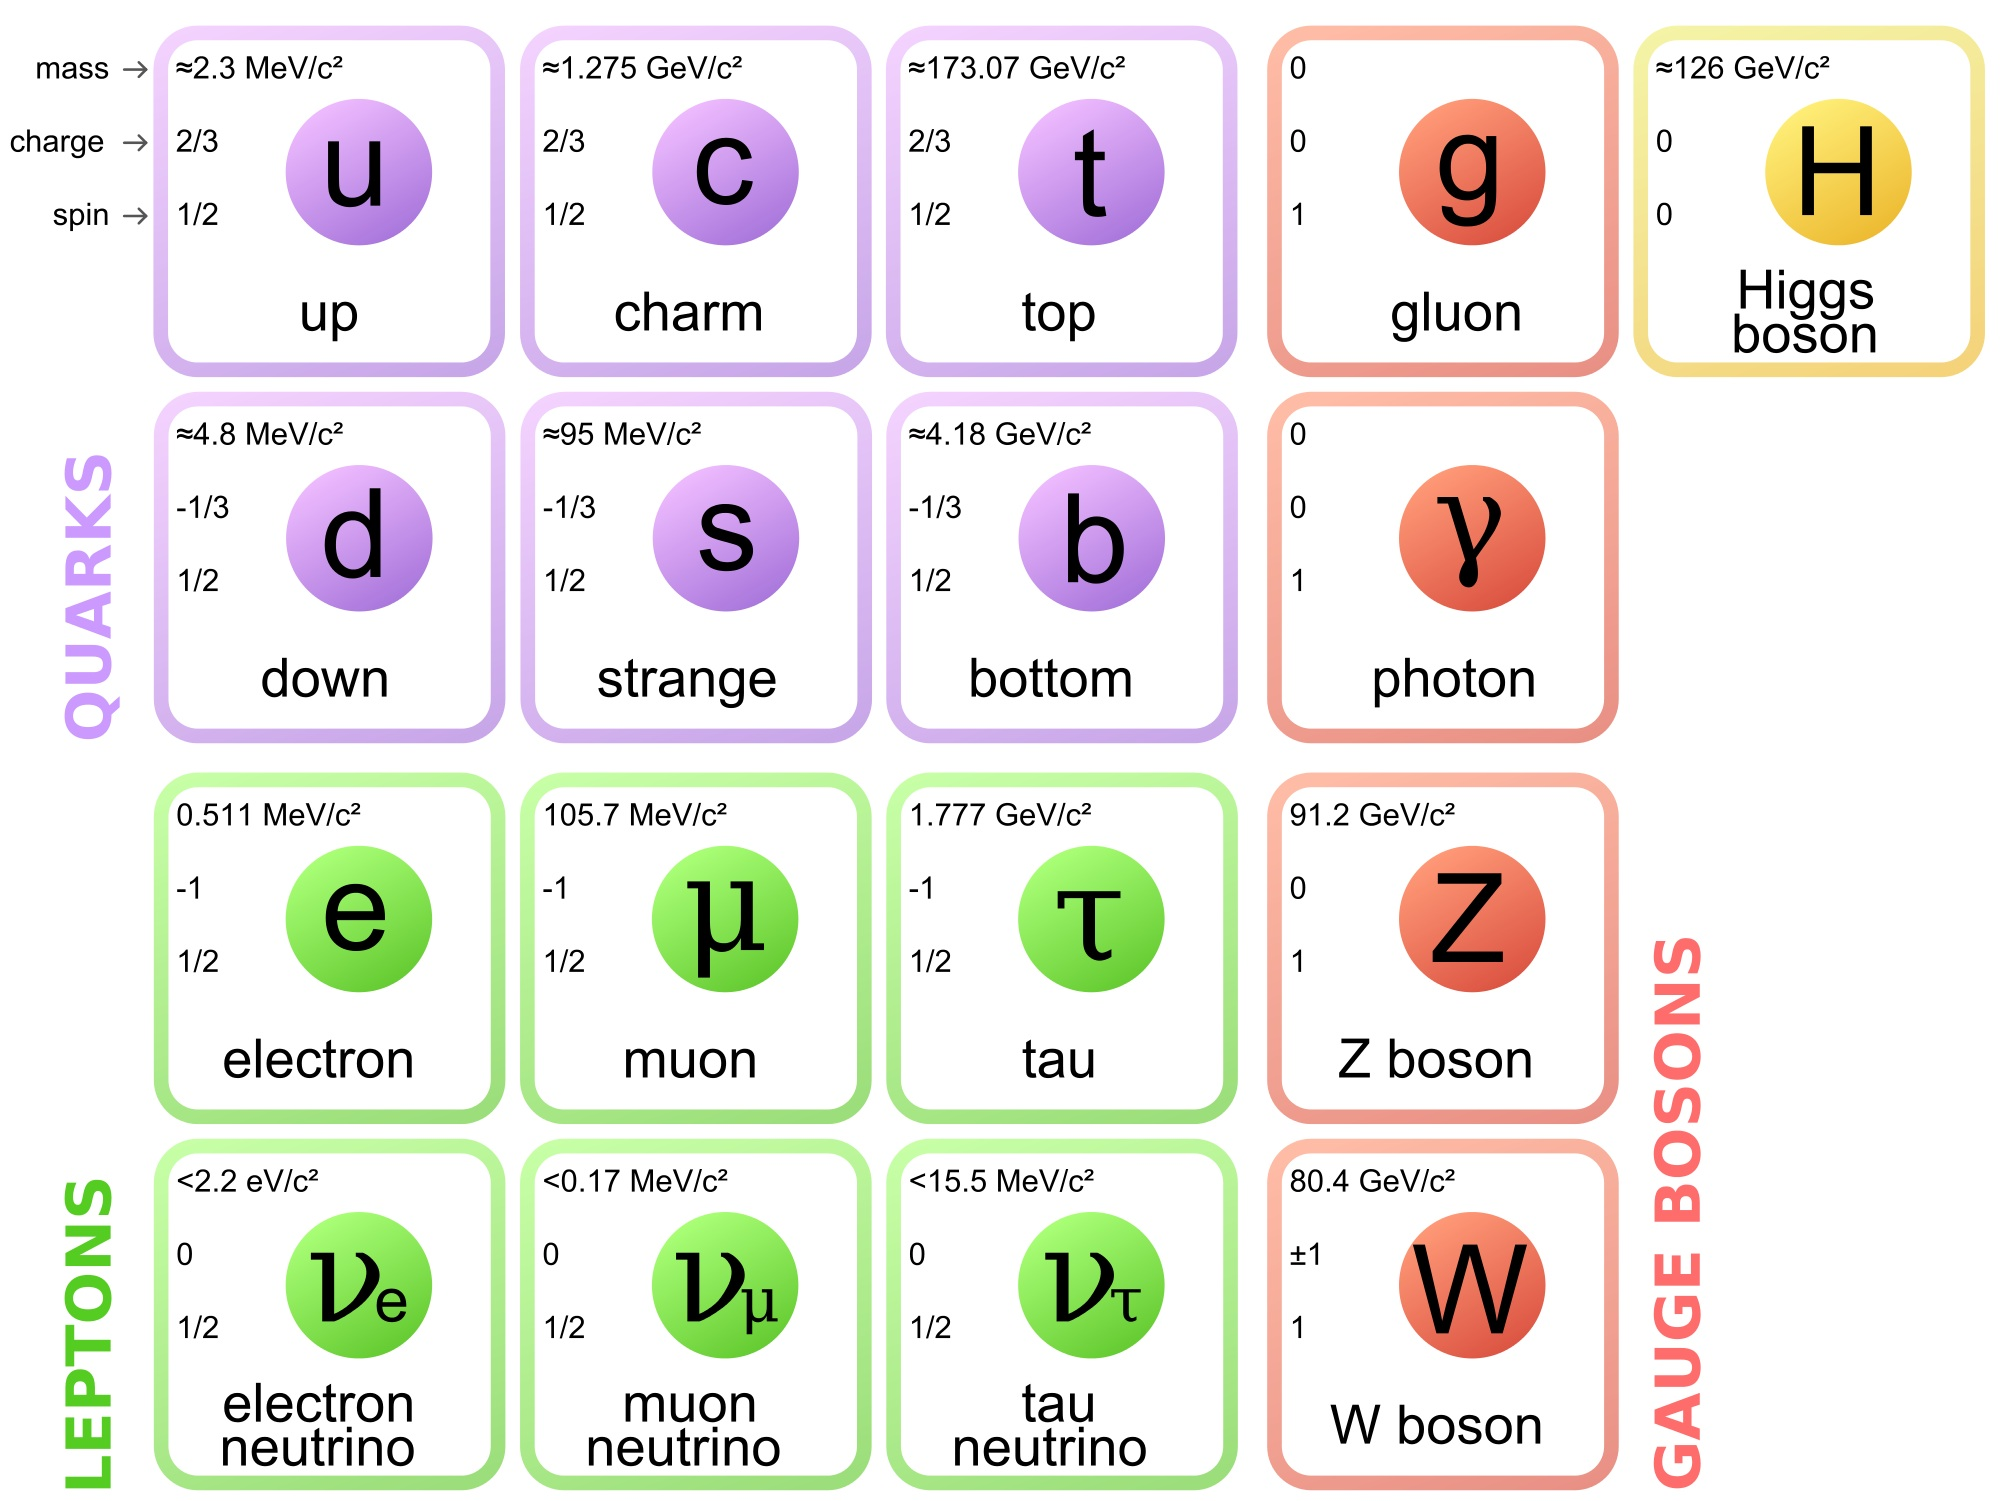
\includegraphics[width=0.8\textwidth]{SM.jpg}\hfill%
  \caption{The particle content of the Standard Model, showing the fermions divided into 3 generations (columns) on the left and the bosons on the right. The electrical charges are expressed as multiples of the absolute value of the electron charge. Figure taken from~\cite{quantumdiaries}.}
  \label{fig:SM}
\end{figure}

A common characteristic of the fermions is their half-integer spin, in contrast to the integer spin of the force mediators, called bosons. Within the Standard Model, the mediation of the different fundamental interactions is represented by the exchange of these spin-1 gauge bosons, which are summarised in Figure~\ref{fig:SM}. The massless photon mediates the most familiar force, the electromagnetic interaction, which is responsible for light, electromagnetic fields, and chemical reactions. The weak interaction is among other things used to describe the radioactive $\beta$ decay, and is propagated by the neutral massive $Z$ boson and and two charged massive $W$ bosons. Lastly, the strong interaction is carried by massless gluons, keeping the protons and neutrons in the atomic nuclei and holding the quark constituents together. A resulting property of the quarks is that they hadronise, i.e. they cannot exist isolated, but form bound states via the strong interaction. These bound states are referred to as hadrons, and can be made up from three quarks or a quark and an antiquark, respectively called baryons and mesons.

Finally, it is also important to note that for every fermion~$(f)$ there exists an antifermion~$(\bar{f})$, which differs only in electric charge and handedness of spin. When matter and antimatter come into contact they can annihilate, generating energy which can be transformed into other particles.

\subsection{The theoretical framework of the Standard Model}

The Standard Model goes further than merely giving an exhaustive list of elementary particles, it has a supporting theoretical framework formulated as a relativistic quantum field theory. In a quantum field theory, every particle is represented by discrete excitations of a field $\psi(x)$, where $x$ is the space-time coordinate. The interactions and kinematics of this particle are fully determined by the action $S$, which is defined as the integral of the Lagrangian  $\mathcal{L}(\psi(x), \partial^{\mu}\psi(x))$ over the space-time coordinates:
\begin{equation}
 S = \int\mathcal{L}(\psi(x), \partial^{\mu}\psi(x))d^4x.
\end{equation}
The Lagrangian  is a function of the field $\psi(x)$ and its first derivative $\partial^{\mu}\psi(x)$, where $\mu$ represents the index of the space-time coordinate. The physical behaviour of the particles is obtained by following the principle of least action $\delta S =0$, minimizing the action.

In this framework based on the gauge invariance of the Lagrangian under the fundamental symmetries, the interactions between the fermions and bosons follow automatically. This can be illustrated with the following example for invariance under a general local gauge transformation.

As mentioned before, a fermion has a half integer spin and can thus be represented as a complex relativistic spin-1/2 field, called a Dirac spinor:
\begin{equation}
\label{eq:Ldirac}
 \mathcal{L}_{Dirac} = i\bar{\psi}\gamma^{\mu}\partial_{\mu}\psi - m\bar{\psi}\psi,
\end{equation}
where $\gamma^{\mu}$ are the Dirac matrices, and the adjoint field $\bar{\psi} = \psi^{\dagger}\gamma^0$ is the field associated to the antifermion. The imposed local gauge invariance then requires the fermion fields, and the overall Lagrangian, to be invariant under so-called local phase transformations
\begin{equation}
 \psi \rightarrow \psi' = U(x)\psi = e^{i\vec{\alpha}(x)\cdot\frac{\vec{\tau}}{2}}\psi
\end{equation}
where $\vec{\alpha}(x)$ are the space-time dependent rotation parameters in the symmetry group represented by the Lie group generators $\vec{\tau}$. Since the derivative $\partial_{\mu}$ in (\ref{eq:Ldirac}) spoils the invariance of the Lagrangian under a local phase transformation, it is replaced with a covariant derivative 
\begin{equation}
 D_{\mu} = \partial_{\mu} - ig\frac{\vec{\tau}}{2}\vec{A}_{\mu}, 
\end{equation}
restoring the invariance. This however introduces new vector gauge fields $A_{\mu}$, which interact with the fermion fields with a coupling strength $g$. As a result, the Dirac Lagrangian contains an additional term, which describes the interaction between the fermion fields mediated by the gauge fields $A_{\mu}$, and (\ref{eq:Ldirac}) becomes
\begin{equation}
  \mathcal{L}_{Dirac} = i\bar{\psi}\gamma^{\mu}\partial_{\mu}\psi - m\bar{\psi}\psi + g\bar{\psi}\gamma^{\mu}\frac{\vec{\tau}}{2}\psi\vec{A}_{\mu}
\end{equation}

The matrix $U(x)$ which was introduced above, was defined as a general rotation matrix of the symmetry group $SU(N)$. In order to obtain the three fundamental interactions of the Standard Model, the described procedure can be simplified using the corresponding symmetry groups as mentioned below.

\begin{itemize}
 \item[] \textbf{Electroweak theory}\\
 The electroweak interaction describes the electromagnetic and weak interactions, which appear very different at low energies but can be merged into a single electroweak force above the electroweak energy scale. This theory is described by requiring gauge invariance under the $SU(2)_L \otimes U(1)_Y$ symmetry group. This leads to 3 gauge fields $W_{\mu}^{\alpha}$ introduced by the $SU(2)_L$ group, and one gauge field $B_{\mu}$ from the $U(1)_Y$ group. Two coupling constants are introduced, $g_1$ and $g_2$, for $U(1)_Y$ and $SU(2)_L$, respectively. The corresponding observable gauge bosons are then obtained as linear combinations of these fields:
 \begin{equation}
  A_{\mu} = \sin\theta_{\mathrm{W}} \mathrm{W}^3_ {\mu} + \cos\theta_{\mathrm{W}}\mathrm{B}_{\mu},
 \end{equation}
 \begin{equation}
  Z_{\mu} = \cos\theta_{\mathrm{W}} \mathrm{W}^3_{\mu} - \sin\theta_{\mathrm{W}}\mathrm{B}_{\mu},
 \end{equation}
 \begin{equation}
  W_{\mu}^{\pm} = \sqrt{\frac{1}{2}}\left(\mathrm{W}^1_{\mu} \mp i\mathrm{W}^2_{\mu}\right),
 \end{equation}
 where $A_{\mu}$, $Z_{\mu}$, and $W_{\mu}^{\pm}$ are the photon, $Z^0$, and $W^{\pm}$ fields, respectively, and $\theta_{\mathrm{W}}$ is the weak mixing angle defined as $\tan\theta_{\mathrm{W}} = \frac{g_1}{g_2}$.

  \item[] \textbf{\ac{QCD}}\\
 The strong interaction is described by the theory of \acf{QCD} and is represented by the symmetry group $SU(3)$. It describes the interaction between particles that carry a colour charge, which can be red, green, blue, or one of the three corresponding anticolours. There are eight gauge boson fields associated to this group, which are massless and known as gluons. An important aspect which is unique for this interaction is asymptotic freedom, which states that the strong coupling constant, denoted by $\alpha_s$, goes to zero at high energies. Consequently, the strong force becomes stronger as the distance between the strongly interacting quarks and gluons increases. As a result, the quarks and gluons cannot exist independently and are not observed individually, but are instead confined in colour-neutral hadrons. This effect is called confinement.
\end{itemize}
  
At this point the resulting Lagrangian including the three fundamental forces does not contain any mass terms, and so it cannot explain the observed particle masses. Additional mass terms cannot simply be added explicitly because they would break gauge invariance. Instead, a solution to this problem is found by introducing a complex scalar doublet $\phi$ with a non-zero vacuum expectation value (vev) $v$. This breaks the electroweak symmetry and is known as the Brout-Englert-Higgs (BEH) mechanism, postulated in 1964~\cite{Englert:1964et,Higgs:1964pj, Guralnik:1964eu}. The Lagrangian of the Higgs field is
 \begin{align}
   \mathcal{L}_H &= (D^{\mu}\phi)^{\dagger}(D_{\mu}\phi) - V(\phi)\nonumber\\
   &= (D^{\mu}\phi)^{\dagger}(D_{\mu}\phi) +\mu^2\phi^{\dagger}\phi - \lambda(\phi^{\dagger}\phi)^2,
 \end{align}
where $\mu$ is a real constant representing a mass parameter and $\lambda$ is a dimensionless parameter standing for the self-interaction strength. The potential $V$ of the scalar doublet has an infinite set of minima or ground states, and by choosing a ground state and expanding the field around it, the electroweak symmetry is broken. As a result, three of the four original fields of the scalar doublet are absorbed by the massless vector fields of the weak interaction, giving mass to the $W$ and $Z$ bosons:
\begin{equation}
 M_W = \frac{1}{2}vg_2 \qquad M_Z = \frac{1}{2}v\sqrt{g_1^2 + g_2^2}.
\end{equation}
From the remaining field, the $H$ boson arises, acquiring a mass $m_H = \sqrt{2\lambda} v$.

The introduction of mass terms for the fermions also follows from the BEH mechanism, which allows to insert the following gauge-invariant term in the Lagrangian:
\begin{equation}
  \mathcal{L}_{Yukawa} = -Y_{ij}\bar{\psi}_{L,i}\phi\psi_{R,j} + h.c.
\end{equation}
with the $Y_{ij}$ Yukawa matrices. The $L$ and $R$ here denote left-handed and right-handed fermions. This handedness or chirality is defined as $\psi_{L} = \frac{1}{2}(1-\gamma_5)\psi$ for left-handed and $\psi_{R} = \frac{1}{2}(1+\gamma_5)\psi$ for right-handed fermions. The fermion masses then arise from the Yukawa interactions describing the couplings of the fermions with the Higgs field. For massive particles, a reference frame which overtakes the spinning particle can always be found, in which case the particle will seem to move backwards, flipping its helicity\footnote{The helicity is defined as the sign of the projection of the spin vector onto the momentum vector of a particle, left is negative and right is positive.}. This is however not the case for massless particles, which travel at the speed of light. So far only left-handed neutrinos and right-handed antineutrinos have been observed, which would imply that the neutrinos are massless in the Standard Model. This lack of observation can however be explained by assuming these neutrinos are much more weakly coupled.

\subsection{Unanswered questions of the Standard Model}

Although the Standard Model is an extremely successful theory, there are still many questions that remain unanswered, indicating that the Standard Model cannot be a complete theory of nature. A brief description of some of the main questions being asked follows here.
\begin{itemize}
 \item[] \textbf{Grand Unified Theory}\\
 As the weak and electromagnetic interactions were successfully unified into the electroweak one, the idea of representing the three forces of the Standard Model by a single one is envisaged and studied. While this Grand Unified Theory (GUT) could be a first step towards the incorporation of gravity in the Standard Model, it cannot be achieved with the current Standard Model and requires new physics at a very high energy scale.
 
 \item[]\textbf{Baryon asymmetry}\\ 
 This problem refers to the imbalance of matter and antimatter in the universe. While the Big Bang should have produced an equal amount of baryonic and antibaryonic matter, this is not measured in our observable universe. It is assumed that most of the primordial matter and antimatter annihilated, but an imbalance allowed a fraction of the matter to survive. Within the Standard Model, some asymmetry in the production of matter and antimatter could be explained by the CP-violation\footnote{According to Charge Parity (CP) symmetry, the laws of physics should remain identical when converting a particle into its antiparticle and mirroring the space coordinates. However, measurements of e.g. kaon-antikaon mixing show that this symmetry is violated.} of the weak interaction. However, the amount of CP-violation needed to explain the baryon asymmetry is ten times higher than is observed from Standard Model measurements. 
 
 \item[]\textbf{Hierarchy problem}\\ 
%  The hierarchy problem concerns the question why the weak force is so much stronger than gravity. The measured vector boson masses suggest that the electroweak symmetry breaking should occur at an energy scale of $\mu^2 \sim (100$~GeV$)^2$, while the energy regime where gravity becomes comparable to the other forces, called the Planck scale, is of the order of $\Lambda_{Planck} \sim 10^{19}$~GeV. 
 This issue is related to the mystery as to why the Higgs boson mass is so much smaller than the Planck scale. The real physical Higgs boson mass, expressed as $m_{\mathrm{H}}^2 = m_{\mathrm{H, bare}}^2 + \mathcal{O}(\Lambda^2)$, is composed of its bare mass and quantum loop corrections. As the Higgs boson is a scalar particle, the corrections depend strongly on the cut-off scale $\Lambda$, instead of logarithmically as is the case for renormalisable interactions. At the electroweak scale, which is of the order of \SI{100}{GeV}, the corrections are of the same order of magnitude as the bare mass. When going to high energy scales such as the Planck scale however, a divergence occurs. A significant fine-tuning would be needed for the bare mass and the huge quadratic radiative corrections to cancel, in order to obtain the experimentally determined mass of \SI{125}{GeV}. This unnatural amount of fine-tuning is not desirable for any theory. This so-called naturalness problem can be solved by introducing new particles which interact with the Higgs boson in such a way that the correction terms coming from Standard Model particles are partially cancelled.
 
 \item[]\textbf{Neutrino masses}\\ 
 The Standard Model predicts that the neutrinos are massless weakly interacting particles, but observations by the Sudbury Neutrino Observatory~\cite{Ahmad:2002jz} and Super-Kamiokande~\cite{Fukuda:1998mi} collaborations showed the first clear evidence that the neutrinos oscillate from one flavour into another. This can only be explained if the neutrinos differ in mass, implying that at least 2 of the 3 neutrinos are not massless. As mentioned above, neutrino masses can be included in the Standard Model by adding left-handed neutrinos and right-handed antineutrinos, or by extending the model by adding additional heavier particles. These neutrinos or particles have however not been observed yet.
 
 \item[]\textbf{Dark matter and energy}\\
 This mystery arises from cosmological observations which indicate that all known matter described by the Standard Model makes up only 5\% of the matter and energy in the universe. The remaining matter, called dark matter, contributes another 27\%, and will be discussed in more detail in Section~\ref{sec:DM}. In the Standard Model, neutrinos contribute to the dark matter, but their relic density is by far not enough to account for all the dark matter. The last 68\% has been labelled dark energy and is believed to be responsible for the acceleration of the observed expansion of the universe, but remains even more enigmatic as no explanation can be provided by the Standard Model.
\end{itemize}

\section{Dark matter}
\label{sec:DM}

One of the current open questions in particle physics that is not answered by the Standard Model is the existence of dark matter. Many astrophysical observations from gravitational effects (see for instance~\cite{Bertone:2004pz}) show there must be some additional matter in the universe, the so-called dark matter, next to the known matter. Despite this, its precise nature remains as of yet unknown. Countless theoretical models are being constructed in order to explain its origin, and on the experimental side dark matter is being looked for in many different ways, but no observation has been made so far.

\subsection{Observational evidence}

The first hints of dark matter were observed by F. Zwicky~\cite{Zwicky:1933gu} in 1933 by studying the velocity dispersion of galaxies in the Coma cluster. The effect is not only observed for entire galaxies, but also for various luminous objects, such as stars or gas clouds, inside a galaxy. The rotation curves of galaxies have been well studied, and show clear evidence for the existence of dark matter. An example of a rotation curve is shown in Figure~\ref{fig:rotationcurves}, exhibiting a flat behaviour of the rotational velocity at large distances, going even far beyond the edge of the visible disk. However, in Newtonian dynamics the circular velocity is expected to be
\begin{equation}
 v(r) = \sqrt{\frac{GM(r)}{r}},
\end{equation}
where $M(r) = 4\pi\int\rho(r)r^2dr$ with $\rho(r)$ the mass density profile. Assuming $M(r)$ to be constant, the circular velocity is expected to fall like $1/\sqrt{r}$ beyond the disk. Since the measurements show an approximately constant velocity but a dropping visible mass density, this implies the existence of a halo with $M(r) \propto r$ and $\rho(r)\propto1/r^2$. A universal density profile seems to be suggested by the rotation curves of both low and high surface luminosity galaxies, consisting of an exponential thin stellar disk and a spherical dark matter halo with a flat core of radius $r_0$ and density $\rho_0 = 4.5\times 10^{-2}(r_0/\textup{kpc})^{-2/3}\textup{M}_\odot\textup{pc}^{-3}$~\cite{Salucci:2002jg}\footnote{$\textup{M}_\odot$ denotes a solar mass, $2 \times 10^{30}$~kg.}.

\begin{figure}[ht]
  \centering
  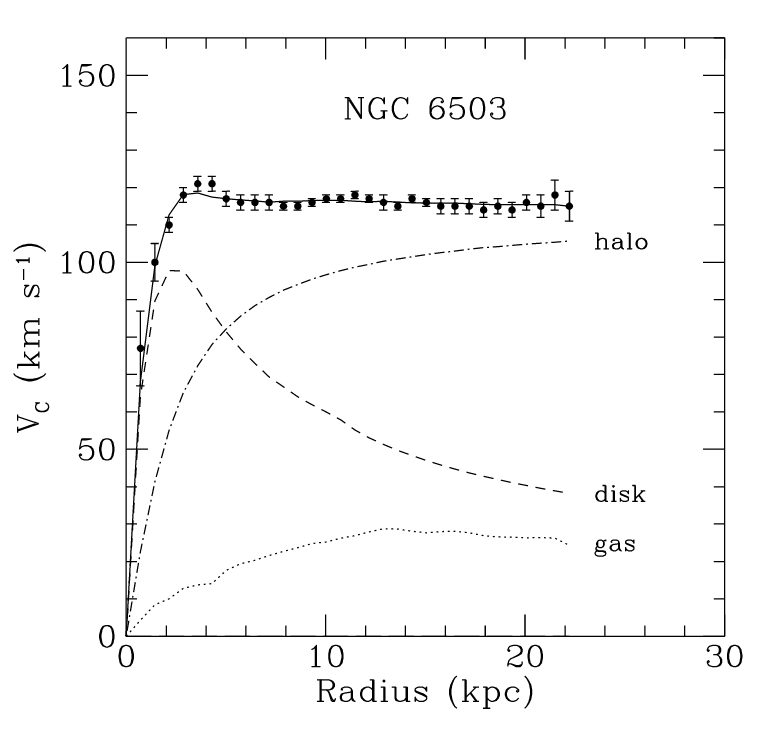
\includegraphics[width=0.6\textwidth]{rotational_curve.png}\hfill%
  \caption{Rotation curve of NGC 6503. The dotted, dashed, and dash-dotted lines show the contributions of gas, disk, and dark matter, respectively. Figure taken from~\cite{Begeman:1991iy}.}
  \label{fig:rotationcurves}
\end{figure}

Another evidence for dark matter comes from the effect of gravitational lensing, allowing to determine the mass of an object regardless of the light it emits. When a distant star or quasar is aligned with a massive compact object, the bending of its light due to the gravitational field of the massive object can 
lead to multiple distorted, magnified, and brightened images, as illustrated in Figure~\ref{fig:gravitational_lensing}. The distortion of the image can then be used to determine the potential well and thus the mass of the heavy object. Yet another way to determine the mass of a cluster of galaxies, next to gravitational lensing and the distribution of radial velocities, is by studying the profile of X-ray emission, tracing the distribution of the hot emitting gas in clusters. In general, these three methods are in reasonable agreement with each other.

\begin{figure}[ht]
  \centering
  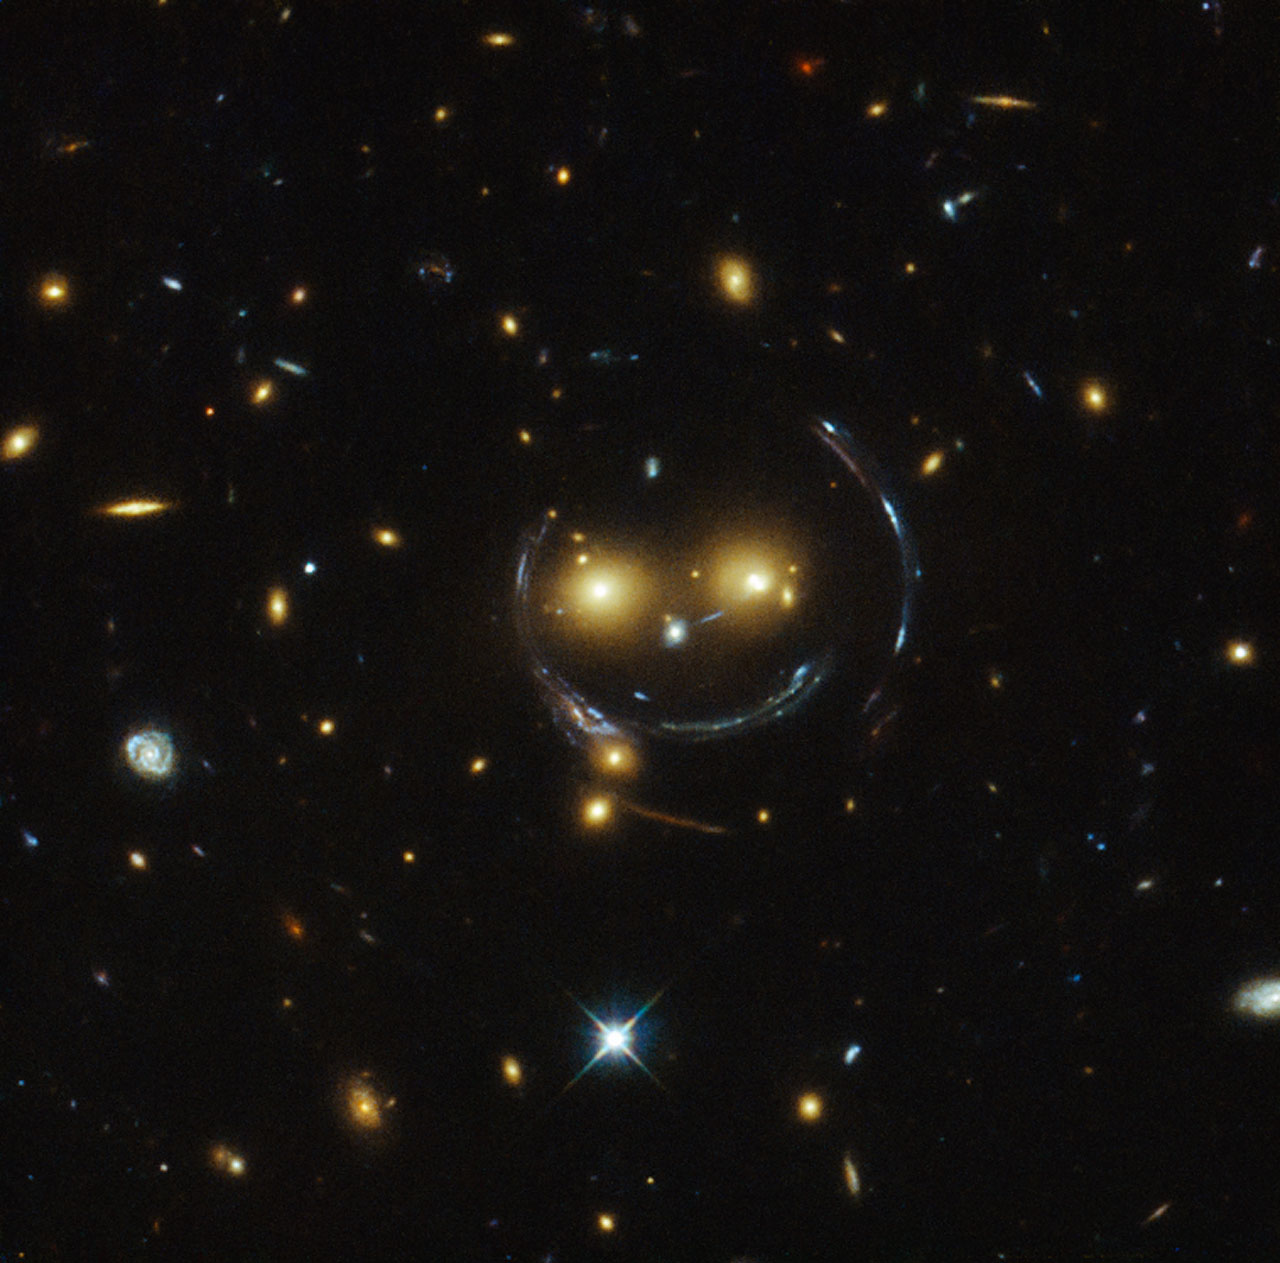
\includegraphics[width=0.65\textwidth]{cat.jpg}\hfill%
  \caption{An example of gravitational lensing showing the ``Cheshire Cat'' image of galaxy cluster  SDSS J1038+4849, taken by the Hubble Space Telescope. Figure taken from~\cite{Belokurov:2008pu}.}
  \label{fig:gravitational_lensing}
\end{figure}

Additionally, at a cosmological level, the analysis of the \ac{CMB} allows to determine the total amount of dark matter in the universe. The existence of this isotropic background radiation was already predicted in 1948, and unintentionally discovered by A. Penzias and R. Wilson in 1965~\cite{Penzias:1965wn}. This relic radiation comes from the propagation of photons in the early universe, once they decoupled from matter. Before this, the photons were energetic enough to ionise hydrogen, creating a plasma of electrons and protons which were unable to combine into hydrogen. As the universe expanded and cooled down, the photons also cooled down enough to let the hydrogen atoms recombine, and the universe became transparent. The photons can then travel freely without scattering off the protons and electrons of the plasma, still carrying information from this surface of last scattering. The \ac{CMB} is now known to be isotropic at the level of $10^{-5}$ and to follow the spectrum of a black body corresponding to a temperature of 2.726~K. However, small anisotropies in the \ac{CMB} have first been observed by the COBE satellite~\cite{Smoot:1992td} and more recently by WMAP~\cite{Komatsu:2010fb} and Planck~\cite{Ade:2013zuv}, as can be seen in Figure~\ref{fig:CMB}. These anisotropies correspond to small thermal variations, and are usually expanded as
\begin{equation}
 \frac{\delta T}{T}(\theta, \phi) = \sum_{l=2}^{+\infty}\sum_{m=-l}^{+l} a_{lm} Y_{lm}(\theta, \phi), 
\end{equation}
where $Y_{lm}(\theta, \phi)$ are spherical harmonics. % EB: sounds a bit slangy
The variance of $a_{lm}$ is given by
\begin{equation}
 C_l =  = \frac{1}{2l+1}\sum_{m=-l}^{+l} 
\left\langle|a_{lm}|^2\right\rangle.
\end{equation}
As the temperature fluctuations appear to be Gaussian, the information contained in the \ac{CMB} anisotropy maps can be condensed into the power spectrum given by the behaviour of $C_l$ as a function of $l$. This is generally represented using $D_l = l(l+1)C_l/2\pi$, as illustrated in Figure~\ref{fig:powerspectrum}.

\begin{figure}[ht]
  \centering
  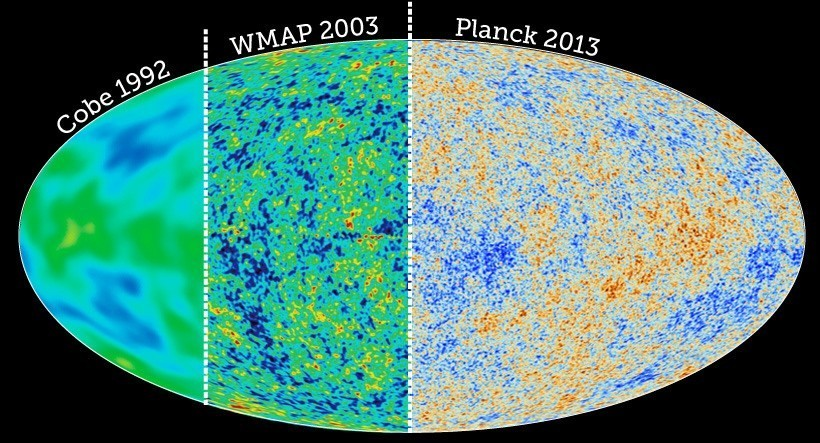
\includegraphics[width=0.8\textwidth]{cmb1.jpg}\hfill%
  \caption{The \ac{CMB} temperature fluctuations obtained from the COBE, WMAP, and Planck data. Figure taken from~\cite{CMB}.}
  \label{fig:CMB}
\end{figure}

\begin{figure}[ht]
  \centering
  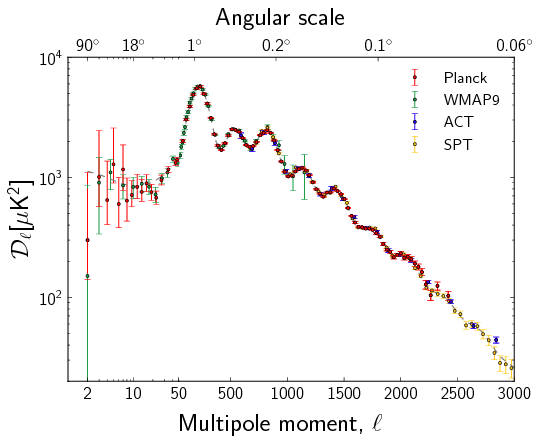
\includegraphics[width=0.8\textwidth]{power_spectrum.png}\hfill%
  \caption{The observed power spectrum of the \ac{CMB} anisotropies. The horizontal axis is logarithmic up to $l = 50$ and linear beyond. Figure taken from~\cite{Ade:2013sjv}.}
  \label{fig:powerspectrum}
\end{figure}

The \ac{CMB} anisotropies are caused by acoustic oscillations arising from the conflict between the gravitational pull from baryons and dark matter and the repulsive force due to the radiation pressure from the photons. One popular model to describe and interpret these observations is the $\Lambda$CDM model. CDM stands for cold dark matter, indicating that in this model the dark matter particles are moving slowly compared to the speed of light, while the $\Lambda$ represents the cosmological constant, which is associated with the vacuum energy or dark energy that is used to explain the accelerating expansion of space. The $\Lambda$CDM model is compatible with a number of observations beyond the \ac{CMB} fluctuations, such as the large scale structure in the distribution of galaxies, the relative abundance of light nuclei, and the accelerating expansion of the universe which is observed from the red shift of well-known spectral absorption or emission lines in the light of distant galaxies. Using the $\Lambda$CDM model to fit the power spectrum of the \ac{CMB} anisotropies, the multiple peaks in the spectrum can be interpreted. The angular scale of the first peak can be used to determine the curvature of the universe. The second peak determines the reduced baryon density and the third peak can be used to retrieve information about the dark matter density. From the analysis of the Planck data the abundance of baryons and matter in the universe is determined to be
\begin{equation}
 \Omega_b h^2 = 0.02205 \pm 0.00028 \qquad \Omega_M h^2 = 0.1423 \pm 0.0029
\end{equation}
This result shows that only about 15\% of the matter in the universe is made up from the ordinary known matter, and the remaining 85\% is called dark matter.

Hot dark matter (HDM), in contrast to CDM, is disfavoured as it is not compatible with the observed small scale structure formation in the universe. Due to the high velocity of the HDM particles, they cannot form clumps as small as galaxies, but would correspond to the formation of larger structures that surround an entire cluster of galaxies. However, models with either a mix of hot and cold dark matter, which could explain both small and large scale structure formation, or models assuming warm dark matter are still being considered.

More evidence for dark matter was found from a great variety of data, both on subgalactic and inter-galactic scales. Without discussing them here in detail, a few examples are the velocity dispersions of spiral galaxy satellites, suggesting the existence of dark halos around spiral galaxies extending well beyond the visible disk~\cite{Azzaro:2003hp}, the velocity dispersion of dwarf spheroidal galaxies, implying larger mass-to-light ratios than those observed in our local neighbourhood~\cite{Mateo:1998wg}, and the so-called Oort discrepancy in the disk of the Milky Way, inferring the existence of dark matter from the inconsistency between the amount of stars in the solar neighbourhood and the gravitational potential indicated by their distribution~\cite{Bahcall:1991qs}.

\subsection{Dark matter models}

There are two main categories of models that can explain the astrophysical observations detailed in the previous section. The models either predict candidates for a new type of matter, or propose modifications to the laws of gravity which could explain the observations at large scales. An example of theories in the latter category is Modified Newtonian Dynamics (MOND)~\cite{Milgrom:1983ca,Milgrom:1983pn,Milgrom:1983zz}. While Newton's laws of gravity have been widely tested for large accelerations, they have never been validated for objects that have an extremely low acceleration, such as stars in the outer parts of galaxies. The included modifications result in a rotation velocity which is independent of the distance to the centre of the galaxy, corresponding to a flat rotation curve. These non-relativistic models have also been extended by inserting them in relativistic theories, resulting for example in a model called TeVeS~\cite{Bekenstein:2004ne}. As a result, this model can also explain observations from gravitational lensing and structure formation. However, it still faces problems to explain the observed \ac{CMB} anisotropies. A more recent alternative theory is based on entropic gravity and describes emergent gravity~\cite{Verlinde:2016toy}.

As these theories are often not complete or are unable to explain all the astrophysical observations, the models focussing on a new type of matter to explain the observed phenomena are usually preferred. Since very little is know so far concerning the nature of dark matter, a multitude of dark matter candidates are discussed in the literature. Without attempting to be complete, a list is given and a few of the more popular candidates are briefly covered here.

\begin{itemize}
 \item[] \textbf{Standard Model neutrinos}\\
	As mentioned before, the Standard Model could explain the existence of dark matter with the already observed neutrinos. However, it can be shown~\cite{Bergstrom:2000pn} that their total relic density is predicted to be 
	\begin{equation}
	 \Omega_{\nu}h^2 = \sum_{i = 1}^3 \frac{m_i}{93\ \mathrm{eV}},
	\end{equation}
	taking the sum over the 3 neutrino flavours. Currently, the most stringent upper bound on neutrino masses is
	\begin{equation}
	 m_{\nu} < 2.05\ \text{eV \hspace{.3cm} at 95\% CL}
	\end{equation}
	obtained in tritium $\beta$-decay experiments at Troitsk~\cite{Lobashev:2003kt,Aseev:2011dq} and Mainz~\cite{Kraus:2004zw}. Since the mass difference between the 3 neutrinos must be very small to explain solar and atmospheric neutrino anomalies~\cite{GonzalezGarcia:2002dz}, this mass limit applies to the three mass eigenvalues, implying an upper bound on the total neutrino relic density of 
	\begin{equation}
	  \Omega_{\nu}h^2 \lesssim 0.07.
	\end{equation}
	This shows that Standard Model neutrinos are not abundant enough to be the dominant component of dark matter.
	
 \item[] \textbf{Sterile neutrinos}\\
         Proposed in 1993 by Dodelson and Widrow~\cite{Dodelson:1993je}, these hypothetical particles are similar to the Standard Model neutrinos, but without Standard Model weak interactions, except for mixing. The analysis of their cosmological abundance and the study of their decay products places stringent constraints on the sterile neutrinos. Light neutrinos with masses below a few keV would for example be ruled out~\cite{Yoshida:2003rm}.
         
 \item[] \textbf{Axions}\\
         These particles were originally introduced to solve the problem of the apparent absence of CP-violation by the strong interaction, and have often been discussed as dark matter candidates. They are expected to interact extremely weakly with Standard Model particles. Furthermore, observations from laboratory searches, stellar cooling, and the dynamics of supernova 1987A constrain the axion mass to be very small, of the order of or below \SI{0.01}{eV}~\cite{Rosenberg:2000wb}. More recently, axions also appear as dark matter candidates in so-called fuzzy dark matter scenarios as an intriguing alternative to cold dark matter, which is not very successful at scales of about \SI{10}{kpc} or less, due to the difficulty of modelling processes such as star formation. This alternative is for example in better agreement with some of the observations that are inconsistent with simple predictions from the $\Lambda$CDM model, such as the absence of dark matter cusps at the centre of dark matter dominated galaxies or the ``missing satellite'' problem~\cite{Klypin:1999uc,Moore:1999nt}. In this type of model, the axion mass is expected to be of the order of $10^{-22}$ to $ 10^{-21}\SI{}{eV}$. More details on the motivation and the astrophysical signatures can be found in~\cite{Hui:2016ltb}.
         
 \item[] \textbf{Massive primordial black holes}\\
	 Primordial black holes are a hypothetical type of black holes, formed during an inhomogeneous phase of the Big Bang. First proposed by Stephen Hawking in 1971~\cite{Hawking:1971ei}, they are good dark matter candidates belonging to the class of massive compact halo objects (MACHOs). While they are stable, have non-relativistic velocities, form very early in the universe, and are nearly collision-less, tight limits on their abundance exist from various observations, excluding them as dominant dark matter candidates for most of the preferred mass range. Nevertheless, the recent detection of gravitational waves from merging black holes by the LIGO and VIRGO experiments~\cite{Abbott:2016blz} could point to the existence of primordial black holes~\cite{Sasaki:2016jop}, and even to a scenario where dark matter is primarily made of primordial black holes~\cite{Clesse:2016vqa, Bird:2016dcv}.
         
 \item[] \textbf{\acs{SUSY} candidates}\\
         Several particles in \ac{SUSY} models can serve as dark matter candidate, such as gravitinos and neutralinos. Gravitinos are the superpartners of the graviton. In some \ac{SUSY} models, they can be the lightest supersymmetry particle and can be stable. While they are very strongly motivated theoretically, they are very difficult to observe, as they only interact gravitationally. The neutralinos are the superpartners of the photon, $Z$ boson, and neutral Higgs bosons. The lightest of the four can be stable and is an excellent dark matter candidate. These dark matter candidates are often called \acp{WIMP}, since they are massive and interact through the weak interaction. As many \ac{SUSY} models predict a new particle with the correct properties and self-annihilation cross section to obtain the correct abundance of dark matter today, a stable supersymmetric partner has long been a very plausible dark matter candidate and a lot of experimental effort has been made to detect it.
         
 \item[] \textbf{\acp{WIMP}}\\         
         A prevalent assumption is that dark matter particles are a relic from the early universe, when all particles were in thermal equilibrium. At those high energies the dark matter particles and antiparticles could be formed by sufficiently energetic lighter particles, and they would annihilate back into these lighter particles as well. However, as the universe expanded and cooled down, the thermal energy of the lighter particles became insufficient to form dark matter particle-antiparticle pairs. The annihilation of the dark matter particles and antiparticles continued however, until the dark matter density decreased considerably and the interaction between the dark matter particles stopped. The number of dark matter particles would remain constant from that moment on, which is referred to as ``freeze-out''. This process is illustrated in Figure~\ref{fig:freezeout}.

\begin{figure}[ht]
  \centering
  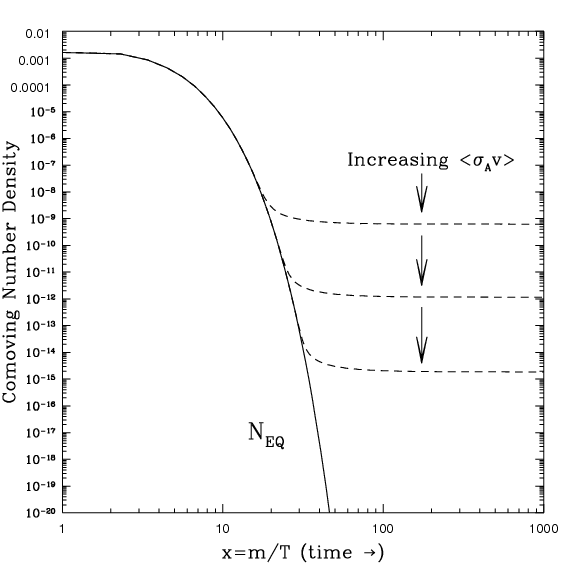
\includegraphics[width=0.7\textwidth]{freezeout.png}\hfill%
  \caption{The evolution of the number density of a thermal relic in time, showing the dropping number density and the freeze-out where the density becomes constant, due to the universe expanding and cooling down. Figure taken from~\cite{Hooper:2009zm}.}
  \label{fig:freezeout}
\end{figure}

	 When the temperature in the universe is lowered below the dark matter mass, the dark matter abundance freezes out to a value which is suppressed by $e^{-\frac{m_{\chi}}{T}}$, and the number density of the dark matter is given by:
	 \begin{equation}
	  n = \left(\frac{m_{\chi}T}{2\pi} \right)^{\frac{3}{2}} e^{-\frac{m_{\chi}c^2}{kT}},
	 \end{equation}
	 with $m_{\chi}$ the dark matter mass and $T$ the temperature of the universe. However, as the universe is expanding at a rate given by the Hubble parameter $H$, the freeze-out will occur when the annihilation rate becomes smaller than the expansion rate of the universe. The annihilation rate of the dark matter particles is given by $n\sigma v$, with $\sigma$ the annihilation cross section which depends on the dark matter model parameters, and $v$ the relative velocity of the two colliding dark matter particles. The resulting relation is quantified by the Boltzmann equation:
	 \begin{equation}
	  \dot{n} + 3Hn = \langle \sigma v \rangle \left(n_{EQ}^2 - n^2\right),
	 \end{equation}
	 with $n_{EQ}$ the number density at equilibrium. Particles with a larger interaction cross section would then continue to annihilate for a longer period of time and would be less abundant. 
         
         The interaction cross section of the annihilating dark matter particles can be inferred from the current estimates of the dark matter abundance in the universe, and can in this case not be larger than the cross section of the weak interaction. According to this model, \acp{WIMP} would be the perfect candidates for dark matter. In general, they are hypothetical new elementary particles that interact gravitationally and through any other force which is as weak or weaker than the Standard Model weak interaction, and they could have been produced thermally as described in this model. Since \acp{WIMP} have a relatively large mass, they would also constitute cold dark matter, which would fit the observed large scale structure of the universe. The coincidence of \acp{WIMP} fitting so well into this model and corresponding to the current observations is known as the ``\ac{WIMP} miracle''.
         
\end{itemize}

Many more dark matter candidates are discussed in literature, such as but not limited to heavy fourth generation neutrinos~\cite{Kainulainen:2002pu}, Kaluza-Klein states in ADD~\cite{ArkaniHamed:1998rs} or RS~\cite{Randall:1999ee} extra dimensions models, superheavy dark matter or Wimpzillas~\cite{Kolb:1998ki}, self-interacting dark matter~\cite{Spergel:1999mh}, charged massive particles (CHAMPs)~\cite{DeRujula:1989fe}, and Q-balls~\cite{Kusenko:1997si}. More detailed reviews are given in~\cite{Ellis:1998gt,Bergstrom:2000pn,Bergstrom:2009ib}.

\subsection{Detection of dark matter}

The detection of dark matter can be categorised in three groups, based on the diagram shown in Figure~\ref{fig:DM_production}. In the case of direct detection experiments, the studied process is the scattering of dark matter off ordinary matter. Experiments searching for dark matter with the indirect approach look for particles or radiation produced in the annihilation of dark matter particles. Finally, at collider experiments, attempts are made to produce and detect dark matter particles by colliding Standard Model particles at high energies.

\begin{figure}[ht]
  \centering
  \includegraphics[width=0.35\textwidth]{DM_production.pdf}\hfill%
  \caption{Diagram illustrating the three used methods to detect dark matter. Indirect detection experiments try to observe Standard Model (SM) remnants of dark matter (DM) annihilation, in the case of direct detection the scattering of dark matter with Standard Model particles is studied, and at colliders one tries to produce dark matter from Standard Model particles.}
  \label{fig:DM_production}
\end{figure}

\subsubsection{Direct detection experiments}

This category of experiments is based on the fact that if our galaxy is filled with a static halo of dark matter particles, then many of them should pass through the Earth as it rotates around Galactic Center, and they could be detected by looking for the interaction of such particles with matter. This is for example done by recording the recoil energy of nuclei when \acp{WIMP} scatter off them. In order to determine the expected rate of events per unit detector material mass, the \ac{WIMP}-nucleon scattering cross section and the density and velocity distribution of the \acp{WIMP} in the solar neighbourhood are needed.

There are several types of scattering processes which can be classified according to two relevant characteristics: elastic or inelastic scattering and spin-dependent or spin-independent scattering. In the case of elastic scattering, the \ac{WIMP} simply scatters off a nucleus as a whole, causing it to recoil. The recoil energy spectrum can then be measured by detecting the emitted scintillation light with very sensitive detectors or by measuring very small temperature changes due to crystal vibrations. Taking a Maxwell-Boltzmann velocity distribution with as characteristic velocity our galactic rotation velocity of about 270 km/s, the recoil spectrum is exponential with typical energies of $\left\langle E \right\rangle \sim 50$~keV. This range of energies is easily detectable by current experiments, which can detect recoils as low as 1-10~keV. Instead, when the \ac{WIMP} scatters inelastically, it interacts with the orbital electrons of the target, exciting the electrons or ionising the target. Differently, the \ac{WIMP} could also excite the target nuclei, which would then emit a photon about a nanosecond after the observed recoil. This signature has, however, to compete with the background from natural radioactivity.

The spin dependence or independence of the scattering depends on the coupling of the \acp{WIMP} to the Standard Model particles. Spin-dependent interactions result from couplings to the spin content of a nucleon, yielding cross sections that are proportional to J(J+1) instead of the number of nucleons. For spin-independent interactions, the cross section instead increases considerably with the mass of the target nuclei. The sensitivity for spin-independent scattering is therefore much enhanced over the spin-dependent one in experiments which use heavy atoms.

Numerous direct detection experiments are currently operational or in development. They use one or more techniques to measure the nuclear recoil, by detecting the scintillation light, the change in temperature, or the ionisation. Some experiments also try to separate the \ac{WIMP} signatures from the background by looking for an annual modulation in the rate, which arises due to the Earth's movement around the Sun. This effect causes the Earth to have a relative velocity with respect to the galaxy's reference frame, given by 
\begin{equation}
v_E = 270\mathrm{km/s}\left(1.05+0.07\cos(2\pi(t-t_m))\right),
\end{equation}
where the time is in units of years and $t_m$ is approximately the beginning of June. As a result, a small variation of about 7\% in the \ac{WIMP} flux can be measured in the direct detection rate. 

Currently, there is some tension between the results obtained by the different experiments, as some observations can be interpreted as dark matter signals, while other experiments are ruling out those models. The DAMA experiment for example observes an annual modulation in the event rate, pointing to the existence of \acp{WIMP} scattering elastically off the sodium and iodine nuclei in the detector~\cite{Bernabei:2013xsa}. 
%However, other experiments are in tension with the various dark matter interpretations of this signal. 
% Similarly, the CoGeNT experiment observes an annual rate modulation as well~\cite{Aalseth:2014eft}. The phase of the signal corresponds to the phenomenological expectation for a \ac{WIMP} at the level of $2.2\sigma$, but the amplitude of the signal is a factor 4 to 7 larger than expected. 
Other experiments, such as SuperCDMS~\cite{Agnese:2014aze}, EDELWEISS-III~\cite{Armengaud:2016cvl}, CRESST-II~\cite{Angloher:2014myn}, XENON100~\cite{Aprile:2016swn}, have seen no evidence for dark matter so far and placed limits on many dark matter models, creating a tension with the observed signal at DAMA. For \ac{WIMP} masses above a few GeV, the strongest limit of direct detection experiments for spin-independent interactions is currently given by LUX~\cite{Akerib:2016vxi}. For a spin-dependent \ac{WIMP}-proton cross section, the most stringent limit is set by the PICO experiment~\cite{Amole:2017dex}, while the PandaX experiment places the strongest limit on the \ac{WIMP}-neutron cross section~\cite{Fu:2016ega}. An overview of the existing limits and signal observations is given in Figure~\ref{fig:direct_detection}, showing the mentioned experiments, and a more complete review of the existing direct detection results is given in~\cite{Undagoitia:2015gya}.

\begin{figure}[ht]
  \centering
  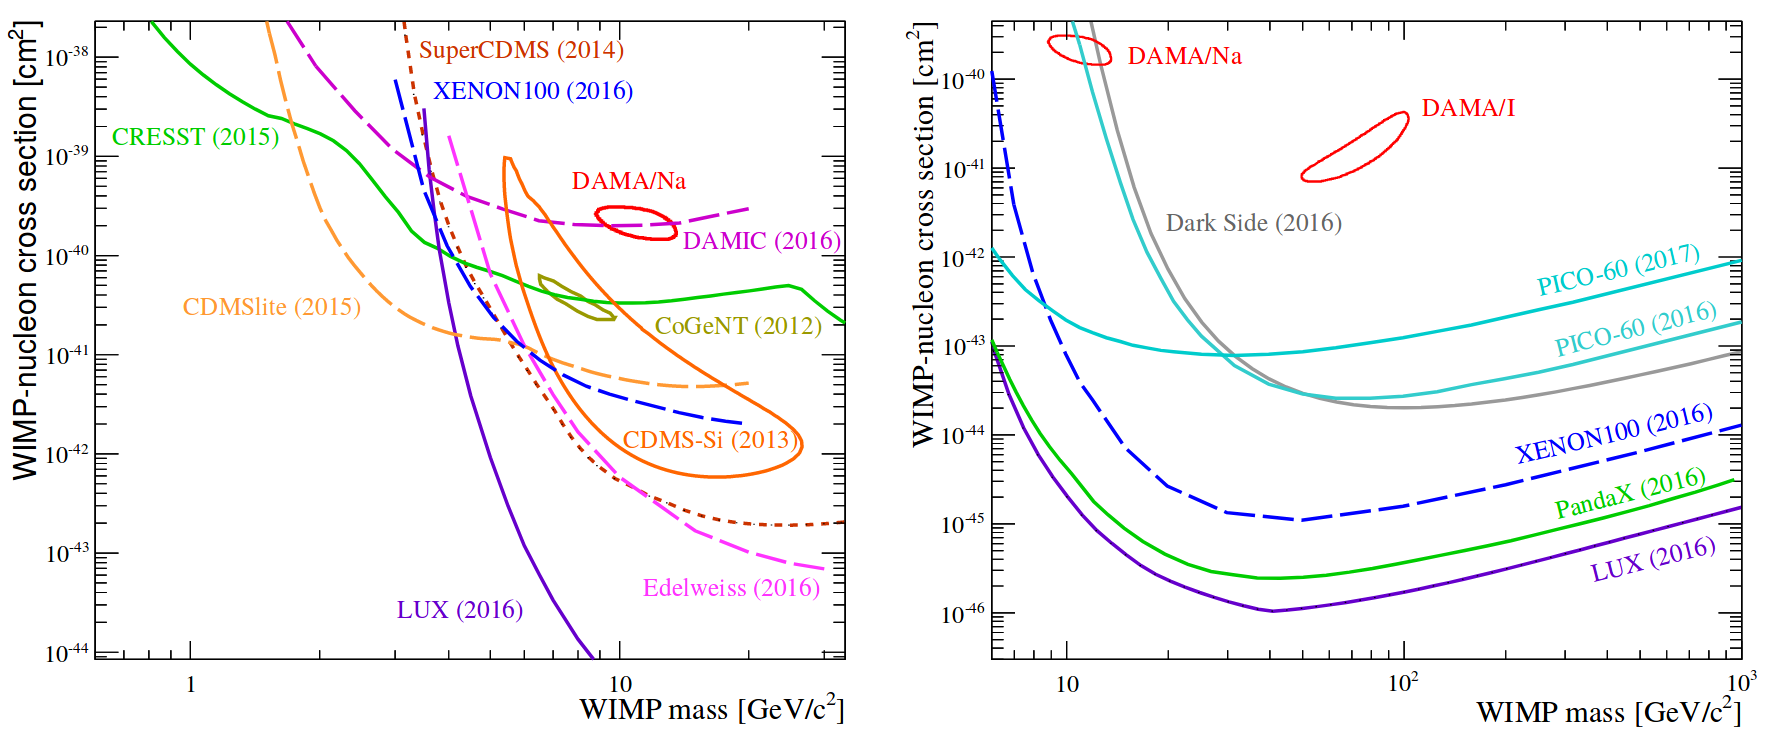
\includegraphics[width=\textwidth]{spinindependent.png}\\
  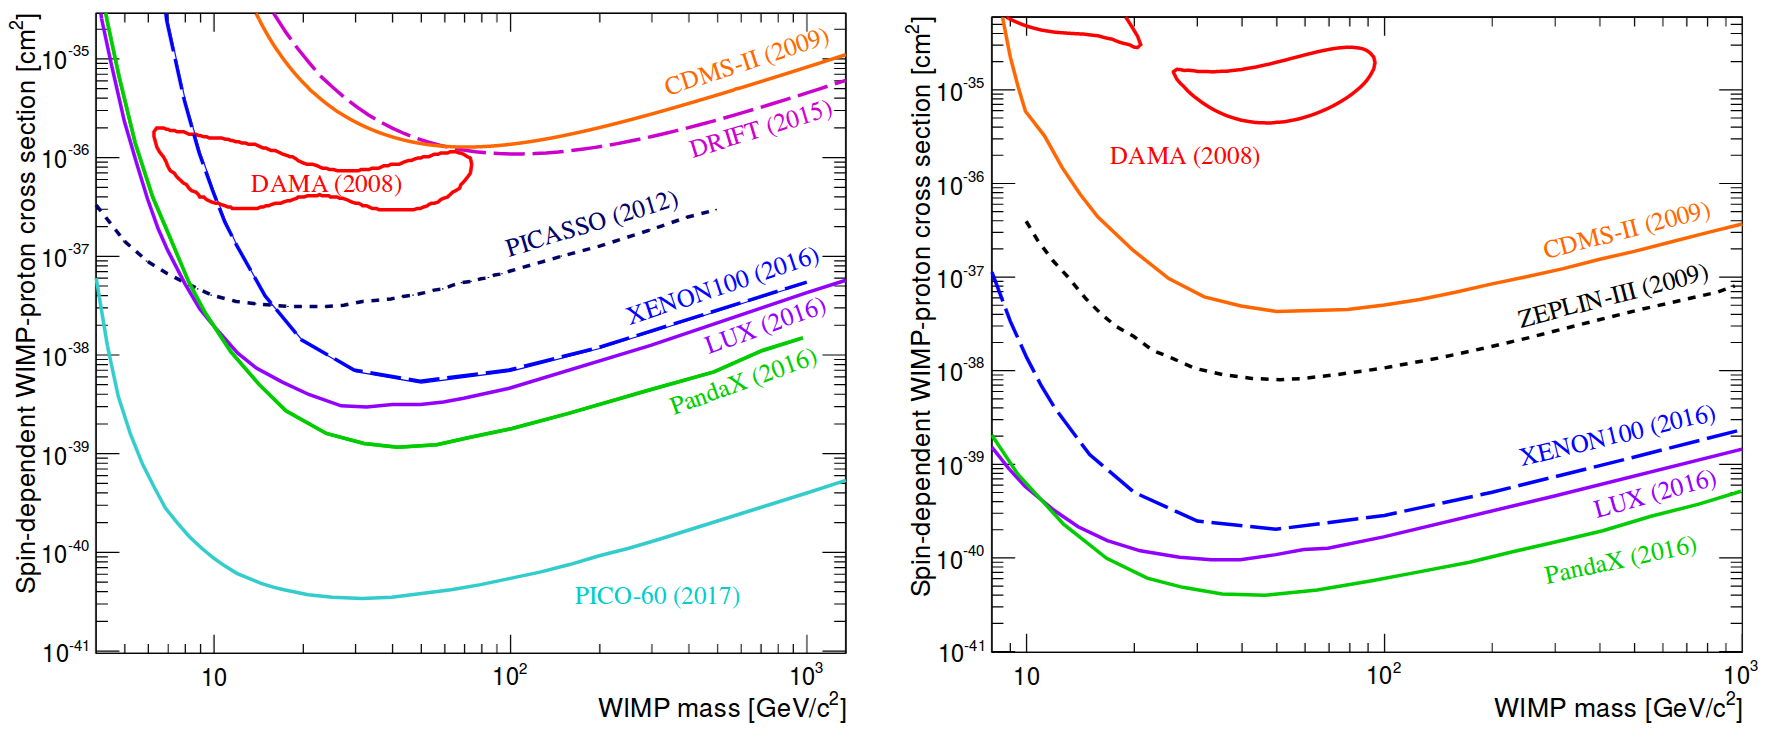
\includegraphics[width=\textwidth]{spindependent.png}\hfill%
  \caption{Overview of the current limits for spin-independent \ac{WIMP}-nucleon interactions at low (top left) and high (top right) \ac{WIMP} masses, spin-dependent \ac{WIMP}-proton interactions (bottom left), and spin-dependent \ac{WIMP}-neutron interactions (bottom right, the y axis title wrongly states \ac{WIMP}-proton cross section). The observed signals from DAMA, CoGeNT, and CDMS-Si are shown as well. Figure taken from~\cite{Undagoitia:2015gya}.}
  \label{fig:direct_detection}
\end{figure}

\subsubsection{Indirect detection experiments}

The indirect detection of dark matter is performed by looking for radiation produced in dark matter annihilations. A reasonable place to look at would then be in regions with large dark matter densities and thus larger annihilation rates, which will result in a higher flux of the studied radiation. Some examples are dense regions of the galactic halo such as the galactic centre, or objects like the Sun or the Earth, which could also capture dark matter particles through scattering with nucleons in their core. In the latter case, only neutrinos would be able to escape those dense objects. Other annihilation products include gamma rays, positrons, and antiprotons.

In order to observe gamma rays directly, the detectors must be placed in space, as photons of the relevant energy range (GeV to TeV) interact with matter via $e^+e^-$ pair production and cannot traverse more than a surface density of about 38~g~cm$^{-2}$. The gamma rays will not reach the ground-based telescopes as the Earth's atmosphere is 1030~g~cm$^{-2}$ thick. Nevertheless, efforts are being made to observe gamma rays indirectly via ground-based experiments as well, by detecting the secondary particles and the Cherenkov light produced by their passage through the Earth's atmosphere. In the energy range between approximately 100~MeV and 100~GeV, gamma ray telescopes on satellites such as the Fermi Large Area Telescope~\cite{Atwood:2009ez} are being used. Above 100~GeV, the ground-based Imaging Air Cherenkov Telescopes such as HESS~\cite{Aharonian:2006pe}, MAGIC~\cite{Aleksic:2011bx}, and VERITAS~\cite{Holder:2008ux} become more adequate.

Neutrinos can also be produced in the annihilation of dark matter particles, but they are considerably more difficult to detect than gamma rays due to their weak interaction with ordinary matter. They are not easily absorbed, which makes it possible to observe them with underground, low-background experiments. Very energetic neutrinos, in the GeV-TeV range, are most easily observed by detecting the Cherenkov light from muons produced through charge current interactions of the neutrinos inside of or close to the detector volume. Two very large neutrino detectors are ANTARES in the Mediterranean Sea~\cite{Collaboration:2011nsa} and IceCube at the South Pole~\cite{Achterberg:2006md}.

Additionally, evidence for dark matter annihilations can also be found by studying the spectra of cosmic positrons and antiprotons. Contrary to neutrinos and gamma rays, these charged particles do not point to their source, as their trajectory is modified by the presence of galactic magnetic fields. Currently, the main detector for positrons and antiprotons is AMS~\cite{Kounine:2012ega}, which is operating on the International Space Station. Until 2016, PAMELA~\cite{Picozza:2006nm} was also active on board of the Resurs-DK1 satellite.

Finally, radio emissions from the galactic halo, and in particular from the galactic centre, can also provide evidence for dark matter annihilation. Electrons and protons produced in dark matter annihilations will emit synchrotron radiation at radio wavelengths as they move through galactic magnetic fields. This type of searches is performed with radio telescopes and belongs to the realm of classical astronomy.

\subsubsection{Collider experiments}

Since dark matter particles are usually assumed to be neutral and to interact only weakly with ordinary matter, they are expected to pass through the detectors at colliders without leaving a signal, similar to neutrinos. These particles can however still be searched for at colliders as well, when they are produced in association with other visible particles which are detected as jets, photons, or charged leptons. The dark matter particles are then observed as missing energy, as they create an imbalance in the net momentum in the transverse plane perpendicular to the colliding beams, which should be zero. One of these flagship analyses is the monojet analysis, looking for dark matter produced together with one or more jets\cite{Sirunyan:2017hci,Aaboud:2016qgg}. Similarly, many more searches are performed at the \acs{CMS} and \acs{ATLAS} experiments at the \ac{LHC} by looking for signatures containing missing energy. Recent summaries are given in~\cite{Kahlhoefer:2017dnp} and \cite{Buchmueller:2017qhf}.

Additionally, other signatures without missing energy can also be used to search for dark matter. If the dark matter particle is produced in a cascade of decays for example, different signatures can be obtained, such as displaced vertices~\cite{ATLAS:2017bvh}, disappearing tracks~\cite{ATLAS:2017bna}, and displaced lepton-jets~\cite{ATLAS:2017lvz}. Furthermore, in dijet searches~\cite{Sirunyan:2017ygf, Sirunyan:2016iap, Aaboud:2017yvp}, resonances in the mass spectrum are being looked for, as this could point to the existence of a new dark matter mediator. If the dark matter particles couple to quarks via a dark matter mediator, this mediator can either decay to a pair of dark matter particles or a pair of Standard model quarks which can be observed as a pair of jets.  Finally, for some particular types of dark matter candidates, such as \acfp{SIMP}~\cite{Bai:2011wy} or \acp{HSCP}~\cite{CMS:2016ybj,Aaboud:2016dgf}, more unusual signatures are expected. This is currently a developing area of dark matter research, and more and more searches looking for new signatures are appearing.

% Many searches for dark matter exist, and the most recent ones are being performed by experiments at the \ac{LHC}. 
In Figures~\ref{fig:summary_SD} and \ref{fig:summary_SI}, recent limits from dark matter searches at the \acs{CMS} experiment are compared to the direct detection results, for spin-dependent and spin-independent interactions, respectively.

\begin{figure}[ht]
  \centering
  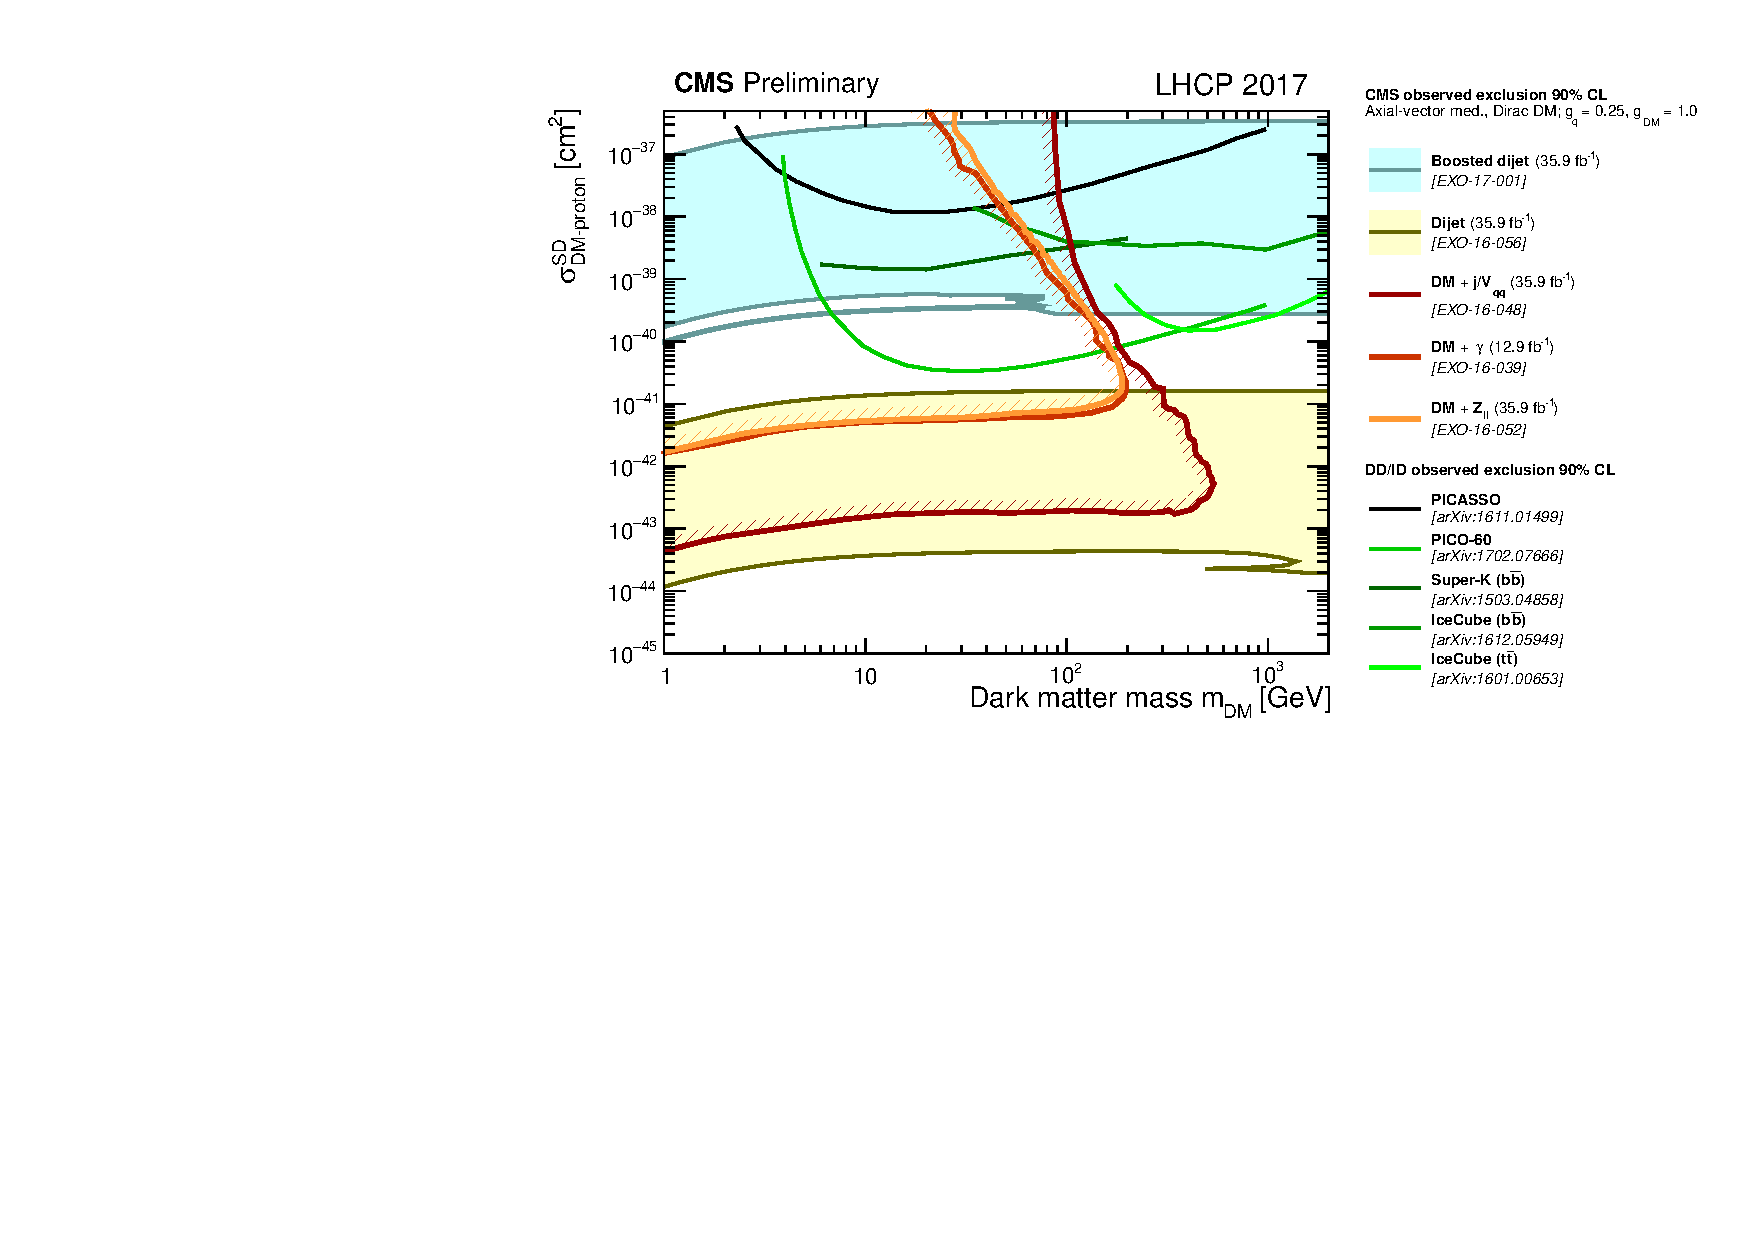
\includegraphics[width=\textwidth]{SD_CMSDD_Summary.pdf}\\
  \caption{A comparison of \protect \acs{CMS} results to direct detection experiments in the $\protect\mathrm{m_{DM}}-\sigma_{\mathrm{SD}}$ plane. The limits are shown at $90\%$ CL. The shown \protect \acs{CMS} contours are for an axial-vector mediator with Dirac dark matter and couplings $g_q=0.25$ and $\protect g_{\mathrm{DM}} = 1.0$. The spin-dependent exclusion contours are compared with limits from the PICASSO and PICO experiments, the IceCube limit for the $\protect t\bar{t}$ and $\protect b\bar{b}$ annihilation channels, and the Super-Kamiokande limit for the $\protect b\bar{b}$ annihilation channel.  It should be noted that the \protect \acs{CMS} limits do not include a constraint on the relic density and also the absolute exclusion of the different \protect \acs{CMS} searches as well as their relative importance will strongly depend on the chosen coupling and model scenario.  Therefore, the shown \protect  \acs{CMS} exclusion regions in this plot are not applicable to other choices of coupling values or models. The IceCube results on the other hand assume the Standard Halo Model and a dark matter annihilation rate of $3 \times 10^{-26} \mathrm{cm}^{-3}\mathrm{s}^{-2}$. Figure taken from~\cite{DMsummary}.}
  \label{fig:summary_SD}
\end{figure}

\begin{figure}[ht]
  \centering
  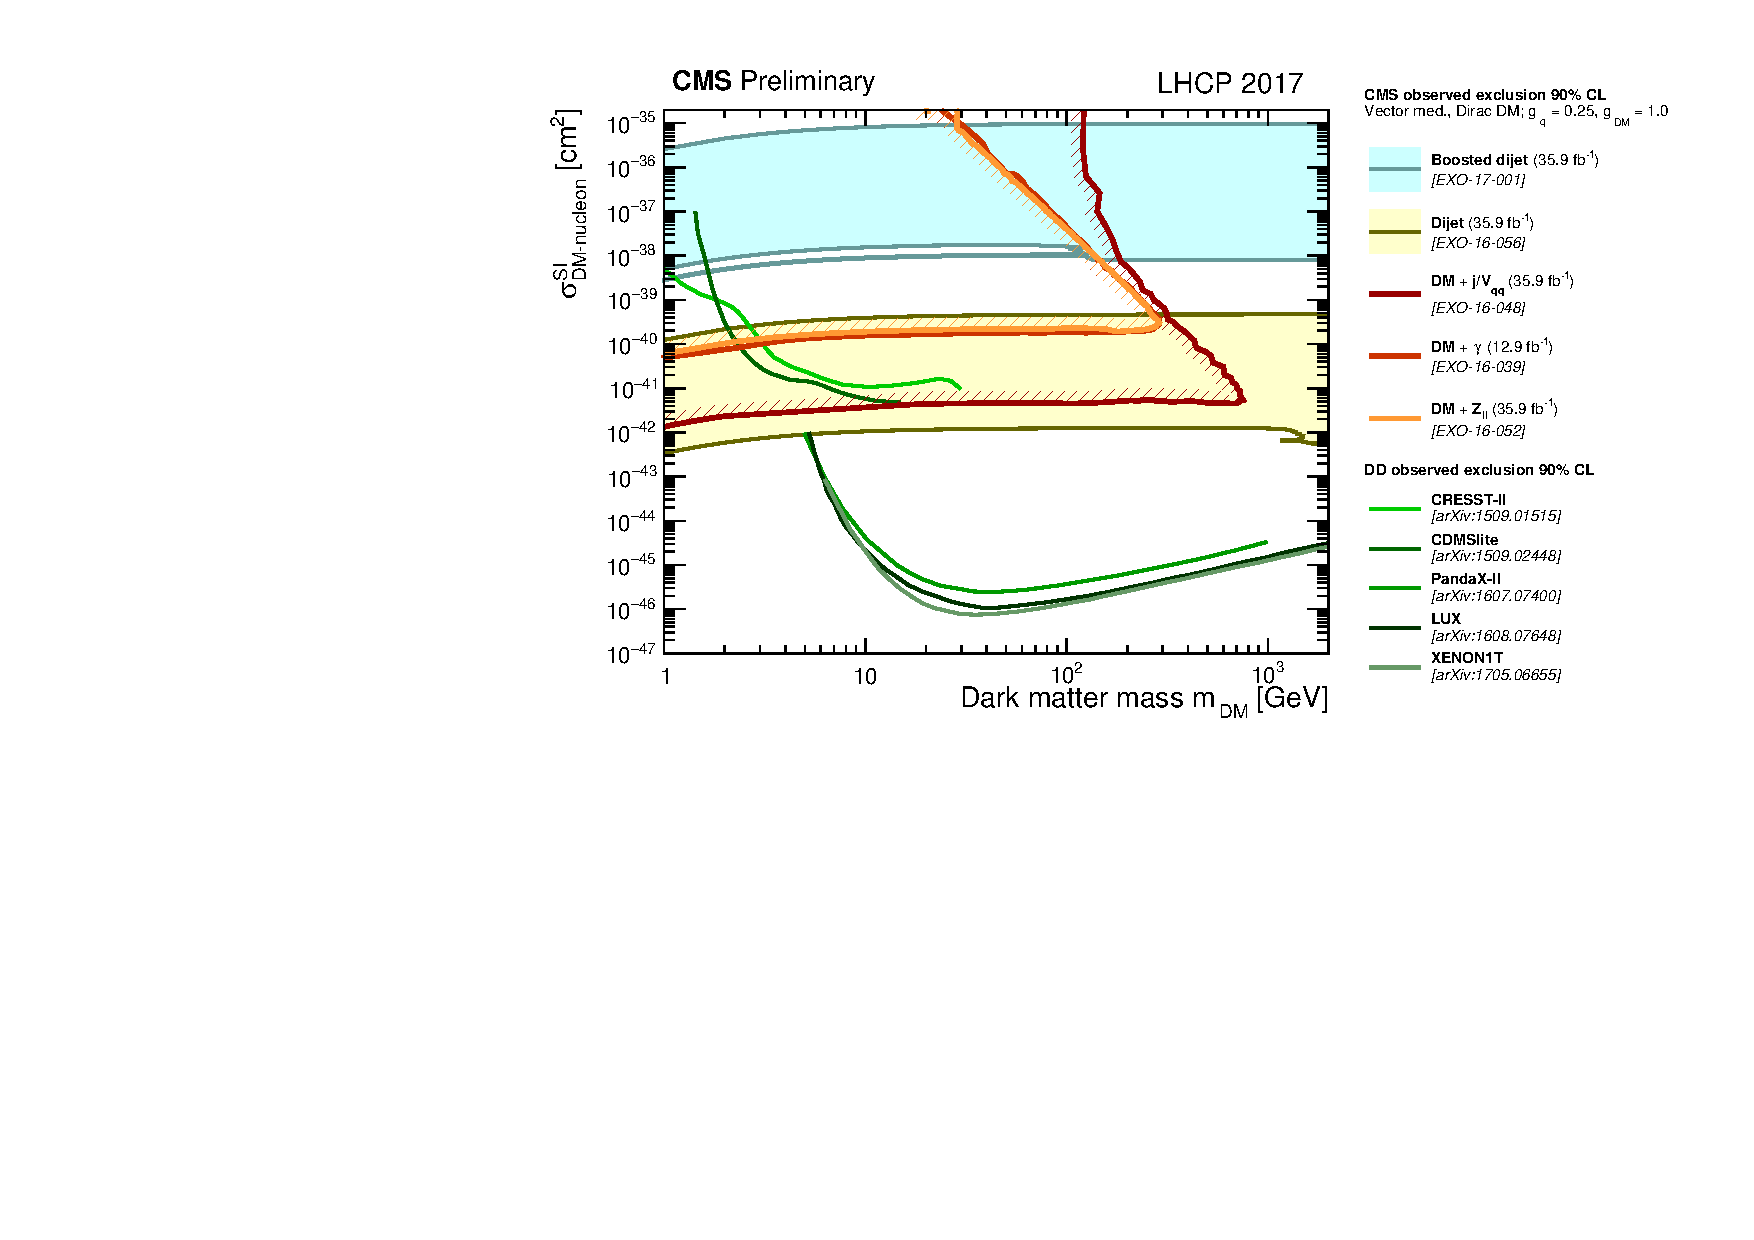
\includegraphics[width=\textwidth]{SI_CMSDD_Summary.pdf}
  \caption{A comparison of \acs{CMS} results to direct detection experiments in the $\protect\mathrm{m_{DM}}-\sigma_{\mathrm{SI}}$ plane. The limits are shown at 90\% CL. The shown \acs{CMS} contours are for a vector mediator with Dirac dark matter and  couplings $g_q=0.25$ and $\protect g_{\mathrm{DM}} = 1.0$. The spin-independent exclusion contours are compared with the XENON1T 2017, LUX 2016, PandaX-II 2016, CDMSLite 2015 and CRESST-II 2015 limits, which constitutes the strongest documented constraints in the shown mass range. It should be noted that the \acs{CMS} limits do not include a constraint on the relic density and also the absolute exclusion of the different \acs{CMS} searches as well as their relative importance will strongly depend on the chosen coupling and model scenario.  Therefore, the shown \acs{CMS} exclusion regions in this plot are not applicable to other choices of coupling values or models. Figure taken from~\cite{DMsummary}.}
  \label{fig:summary_SI}
\end{figure}

\subsection{From EFTs to simplified models}
\label{sec:monojet_models}

In order to efficiently look for dark matter at colliders, effective field theories (EFTs) have been used extensively to model the dark matter signal. The EFT models assume the dark matter production can be described as a contact interaction defined by an effective mass scale and coupling structure. This contact interaction is for example illustrated in Figure~\ref{fig:monojet_diagram} for the monojet final state where the dark matter pair is produced in association with an initial state radiation jet. The resulting signal models can then be classified by coupling structure, and the effective scale $\Lambda$ can be extracted for a specific model, defining both the coupling strength and the scale of the theory. An EFT is characterized by the dark matter mass and the EFT scale. However, this approach has several limitations~\cite{Busoni:2013lha,Busoni:2014sya,Busoni:2014haa}. First, it implicitly assumes that the dark matter production happens through a heavy mediator, which is not resonantly enhanced at the \ac{LHC}. Additionally, for low enough effective scales, the EFT breaks down. Finally, the incompleteness of the EFT makes a comparison with direct detection experiments difficult or inconsistent. Due to the limitations of EFTs, there has been a trend in the past few years to instead use simplified models which allow for a fair comparison to low energy underground direct detection experiments. In a simplified model the effective scale is then replaced by a physical mediator. The resulting models can be classified according to the coupling structure and contain four parameters, namely the dark matter mass, the mediator mass, and the couplings to the Standard Model and the dark matter. These parameters can be scanned for the different types of couplings in order to search for dark matter. The transition to simplified models has been overseen by the joint \acs{ATLAS}/\acs{CMS} dark matter forum~\cite{Abercrombie:2015wmb} by establishing a well defined set of benchmark models to enable the combination of different channels and the recasting of dark matter models against direct and indirect detection searches~\cite{Boveia:2016mrp}.

\begin{figure}[ht]
  \centering
 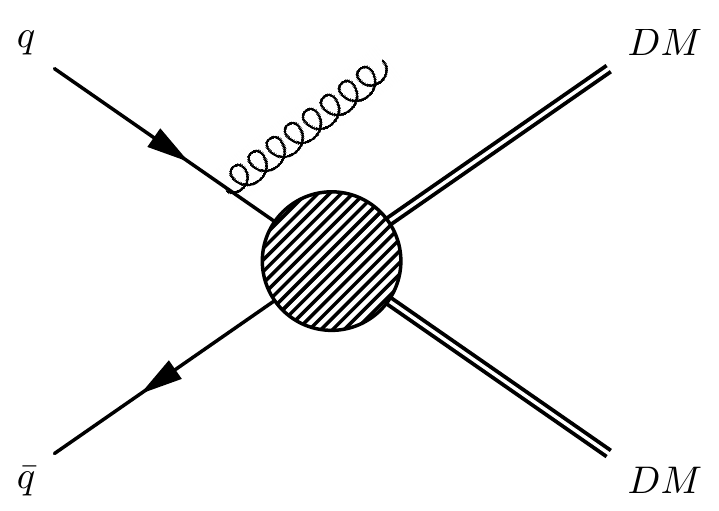
\includegraphics[width=.4\textwidth]{monojet.png} 
 \caption{Illustration of EFT dark matter production in the monojet final state.}
 \label{fig:monojet_diagram}
\end{figure}

In the two dark matter searches covered in this thesis, the results have been interpreted in terms of simplified models. The monojet search described in Chapter~\ref{ch:monojet} includes several simplified models recommended by the dark matter forum. Four types of mediators are considered, i.e. a vector, axial-vector, scalar, and pseudoscalar mediator. In the case of a scalar or pseudoscalar coupling, the production mode is dominated by gluon fusion. As illustrated in the right diagram of Figure~\ref{fig:monojet_diagrams}, the scalar is produced through a $t$ or $b$ quark loop. A Yukawa coupling is assumed for the coupling of the mediator to Standard Model particles, proportional to the mass of the particle. For a vector or axial-vector mediator, the production happens through the fusion of two quarks into a heavy mediator, similarly to the $Z$ and $W$ boson production. The coupling to quarks and potentially leptons is taken to be unity, and universal for all flavours. For all mediator types, the coupling to the dark matter particles is assumed to be unity. In addition, the minimal width assumption is made, implying that the mediator couples to all Standard Model and the dark matter particle and no extra particles are introduced. If such particles would be present, the width would increase and the sensitivity of the analysis would be reduced. A scan is then performed over the mass of the dark matter candidate and the mass of the mediator.

\begin{figure}[ht]
  \centering
 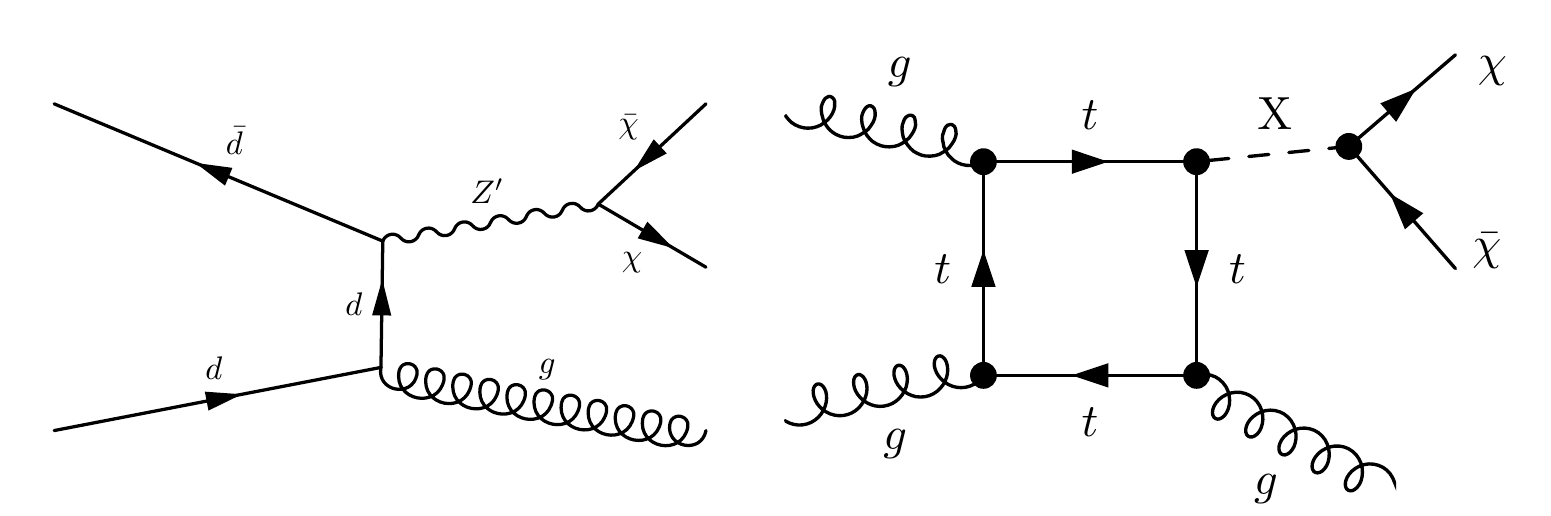
\includegraphics[width=.9\textwidth]{monojet_simplifiedmodel.png} 
 \caption{The vector (left) and scalar (right) production diagrams in the monojet final state.}
 \label{fig:monojet_diagrams}
\end{figure}

For both searches described in this thesis, $s$-channel processes are considered, as shown on the left side of Figure~\ref{fig:channel}. However, in the case of a $t$-channel process illustrated in the right diagram of Figure~\ref{fig:channel}, the simplified model can be characterized using only 3 parameters, since the same coupling appears at both vertices. This type of diagram appears in many studied \ac{SUSY} models, and has recently also been included in the monojet analysis~\cite{Sirunyan:2017jix}.

\begin{figure}[ht]
  \centering
 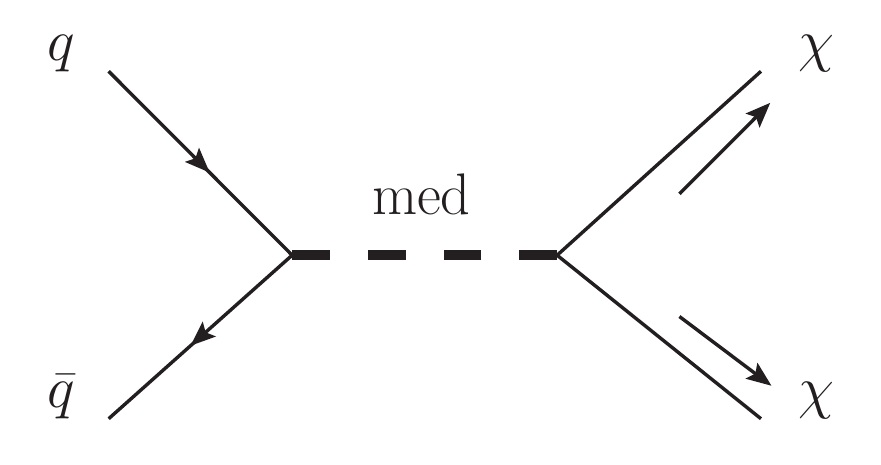
\includegraphics[width=.45\textwidth]{schannel} \hspace{1.5cm}
 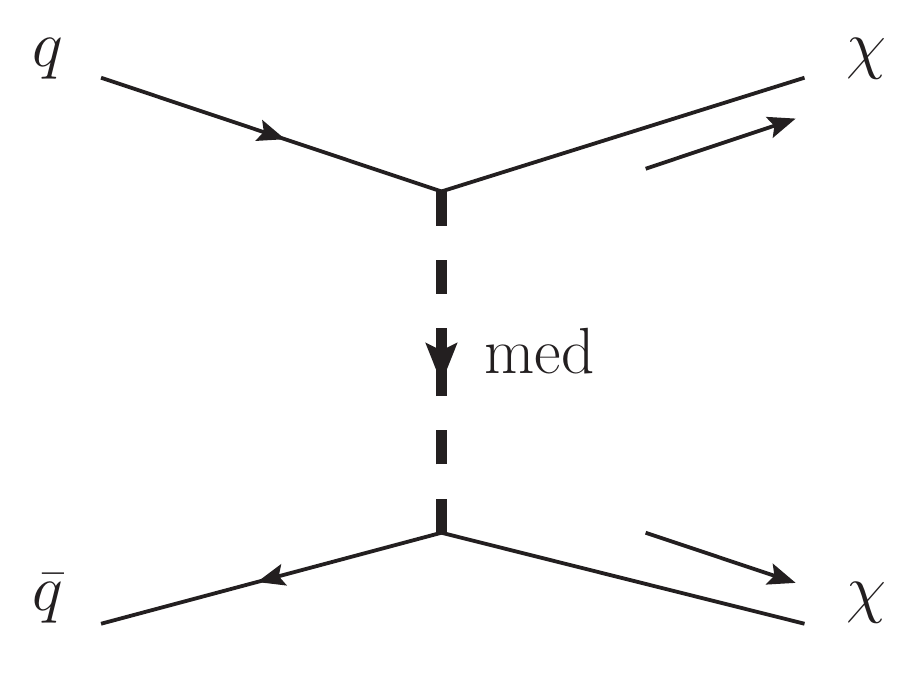
\includegraphics[width=.32\textwidth]{tchannel}
 \caption{Diagrams for dark matter production in simplified models, through an $s$-channel~(left) or $t$-channel (right) process. Figures taken from~\cite{Abdallah:2014hon}.}
 \label{fig:channel}
\end{figure}

% {\color{red} staat enkel in de AN, niet in de PAS...} Furthermore, some non-standard dark matter models are investigated as well in the monojet analysis, namely a complete simplified scalar model, known as the inert two Higgs doublet model and a baryon number violating dark matter model which can explain electroweak baryogenesis~\cite{Goudelis:2013uca,Dutta:2014kia}, known as non-thermal dark matter. In contrast to the simplified models, these theories are completed theories. The first consists of an extended scalar field theory, while the second consists of resonant production induced by flavour changing neutral currents.

% The \acs{SIMP} simplified model on which the trackless jets analysis detailed in Chapter~\ref{ch:SIMPs} is a specific simplified model which is not part of the models recommended by the dark matter forum. It is described in more detail in Section~\ref{sec:SIMP}.

\section{Strongly Interacting Massive Particles}
\label{sec:SIMP}

As no observation of dark matter has been made so far, despite many searches probing the more popular models described in the previous section, many scenarios now venture beyond minimal models or give up basic assumptions for the \ac{WIMP}. In the following model, which is studied in this thesis, the interaction cross section of the dark matter with normal matter is so high that the particles are no longer \acp{WIMP}, but so-called \acp{SIMP}. This model is not part of the models recommended by the dark matter forum, but can also be motivated by the long lasting interest for \ac{SIDM}\footnote{Incidentally, self-interacting and strongly interacting share the same abbreviation, such that SIDM can also stand for strongly interacting dark matter and SIMP for self-interacting massive particles in the literature.} particles with a large cross section~\cite{Spergel:1999mh}, which could help to explain observations that present a challenge for the cold dark matter scenarios, such as the missing satellites or core-cusp problems~\cite{Bullock:2010uy,BoylanKolchin:2011de, Weinberg:2013aya,Famaey:2013ty}. While it is possible to create models with a strongly interacting hidden sector that is weakly coupled to the Standard Model particles, \ac{SIDM} particles that interact rather strongly with the known matter particles can be considered as well. A summary of the existing constraints on this model and a feasibility study of a search for this type of dark matter at colliders were already published in~\cite{Daci:2015hca}, which includes significant contribution by the author.

\subsection{The SIMP simplified model}
\label{sec:SIMP_model}

In this simplified model, the dark matter particles $\chi$ can be produced at the \ac{LHC} in pairs, through a new strong interaction with a new mediator $\phi$, as illustrated in Figure~\ref{fig:diagram}. These \acp{SIMP} are neutral and stable, and are generated off-shell as the mediator is very light, of the order of the pion mass: $m_{\phi} = 140$~MeV. We only consider the case of fermionic candidates, since the bosonic case is ruled out by constraints coming from neutron stars and black holes, as is described in Section~\ref{sec:SIMP_constraints}. Both the cases with a scalar or a vector mediator can be studied, and the corresponding interaction Lagrangian is
\begin{equation} \label{eq:SIMP_lagrangian}
 \mathcal{L}_{\mathrm{int}} = 
 \begin{cases}
  -g_{\chi}\phi\bar{\chi}\chi - g_q\phi\bar{q}q & \text{(scalar mediator)}\\
  -\tilde{g}_{\chi}\phi_{\mu}\bar{\chi}\gamma^{\mu}\chi - \tilde{g}_q\phi_{\mu}\bar{q}\gamma^{\mu}q & \text{(vector mediator)}
 \end{cases}
\end{equation}
with $g_{\chi}g_q,\tilde{g}_{\chi}\tilde{g}_q <0$ to avoid the formation of bound states. For simplicity we assume that the \acp{SIMP} have a universal coupling to quarks, although a flavour dependent coupling could be preferred, as light \acp{SIMP} with a significant coupling to $b$ or $c$ quarks can be constrained by B and D meson phenomenology. \acp{SIMP} lighter than about 5~GeV could for example appear in the decay of $b$ or $c$ quarks, and would be constrained by limits on the invisible decay of B and D mesons.

\begin{figure}[ht]
  \centering
  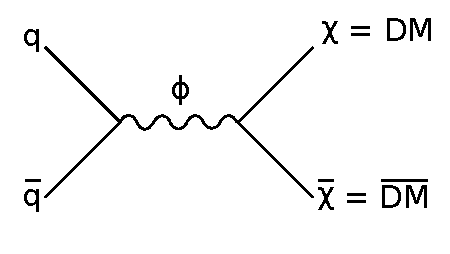
\includegraphics[width=0.45\textwidth]{diagram.pdf}\hfill%
  \caption{Feynman diagram showing the production of a SIMP pair, through a new low-mass mediator.}
  \label{fig:diagram}
\end{figure}

Introducing a new strong interaction between quarks can however modify nuclear potentials. In order to keep the impact small, the mediator is assumed to not modify nuclear potentials by more than $\mathcal{O}(10\%)$, such that $g_{\phi NN} \lesssim 0.3g_{\pi NN}\sim 3$ for a mediator with the mass of a pion, where $g_{\pi NN} \sim 13$ is the effective pseudoscalar pion-nucleon coupling~\cite{Donoghue:1992dd}. The quoted values are however not very precise, as a large spread of values can be found in the literature for meson-nucleon effective couplings, sometimes differing by a factor 2 or more (see e.g.~\cite{Downum:2006re} for comparison). This shows the difficulty of dealing with strong interactions in the framework of effective field theories, which arise because contributions from many mesons need to be taken into account, each of them with a different coupling. No constraints on modified strong interactions at low energies seem to exist in literature so far, however searches at fixed-target experiments do place constraints on the existence of strongly interacting stable neutral particles.

In summary, the model has 4 free parameters: the two couplings, the mass of the mediator $m_{\phi}$, and the mass of the \ac{SIMP} $m_{\chi}$. At the \ac{LHC}, only the product of the couplings appears, while astrophysical observations constrain both the dark matter self-interaction and the interaction with the Standard Model.

\subsection{Experimental constraints}
\label{sec:SIMP_constraints}

Naively, one would expect such an unusual model with strong interactions not to be viable, as various types of experiments and observations set constraints on \acp{SIMP} as dark matter candidates. However, some of these limitations can be avoided by the assumptions in the model described above. The relevant existing measurements are described below, showing there is a still a part of phase space which remained unexplored so far.

\begin{itemize}
 \item[] \textbf{Bound states}\\
Searches for heavy isotopes, in particular heavy water, constrain the formation of bound states between \acp{SIMP} and nucleons, ruling out particles with a mass below 10~TeV for the scenario with \acp{SIMP} as dominant contribution to dark matter. This constraint is evaded by assuming a purely repulsive \ac{SIMP}-nucleon interaction with opposite sign couplings, as is specified in the Lagrangian~(\ref{eq:SIMP_lagrangian}). In the vector mediator case, vector mediators would however couple to the dark matter antiparticles with an opposite charge. This is avoided if no dark matter antiparticles are around, i.e. if the abundance of dark matter is asymmetric. A reason for having asymmetric \acp{SIMP} is that if they are the dominant source of dark matter, then the dark matter abundance is set by either an asymmetry or through a non-thermal mechanism. In the case of a symmetric \ac{SIMP} candidate, the dark matter abundance is determined by thermal freeze-out, and it can only be a sub-dominant component. Additional constraints also exist on the dark matter self-interacting strength from halo shapes and merging galaxies such as the Bullet cluster~\cite{Randall:2007ph, Feng:2010gw}.
% EB: this is a rather dense paragraph that might benefit from a bit more explanation

\item[] \textbf{Earth heating}\\
A second argument for an asymmetric abundance of \acp{SIMP} comes from experiments measuring the heat emitted from the Earth's core. For the typical \acp{SIMP} cross sections, the dark matter particles can be captured by the Earth and accumulate in its core over time. Annihilating \acp{SIMP} would then provide a substantial source of heat and could modify the Earth's heat flow. This can be measured by detectors in deep underground shafts~\cite{Mack:2007xj} and rules out the scenario with symmetric \acp{SIMP}.

\item[] \textbf{Neutron stars and black holes}\\
In the asymmetric scenario, light scalar dark matter particles can however be collected in the cores of neutron stars and cause them to collapse into black holes. Bosonic dark matter candidates are therefore excluded, and we consider only fermionic candidates as mentioned previously.

\item[] \textbf{Direct detection searches}\\
Many bounds on the \ac{SIMP} parameter space come from the direct detection searches as well. Underground experiments, such as CDMS and XENON,
% EB: reference?
place strong constraints at smaller cross sections, about 5 orders of magnitude below the \ac{SIMP} cross section, as can be seen from Figure~\ref{fig:SIMP_summary}. At the higher cross sections considered here, the \acp{SIMP} are stopped by the Earth's atmosphere, and they cannot reach the underground detectors. At higher altitudes however, space or airborne experiments such as RSS~\cite{Rich:1987st}, a balloon-based experiment with a silicon semiconductor detector, and XQC~\cite{Erickcek:2007jv}, a sounding rocket experiment, exclude \acp{SIMP} in some regions of phase space. More details on these constraints can be found in~\cite{Mack:2007xj}, where they have been extensively reviewed.

\item[] \textbf{Nucleosynthesis and cosmic rays}\\
There are also bounds from primordial nucleosynthesis and cosmic rays, reviewed in \cite{Mack:2012ju} and \cite{Cyburt:2002uw}. The protons in cosmic rays can scatter off dark matter particles and create neutral pions, which decay to photons and could be detected in gamma ray telescopes. Although limits have been placed on dark matter-nucleon interactions~\cite{Cyburt:2002uw}, these constraints depend on many assumptions and adopt a form of the dark matter density near the galactic core. Since the considered model describes a nonstandard form of dark matter with a relatively strong interaction with baryons, these densities may be considerably different.

\item[] \textbf{\ac{CMB} and large scale structure}\\
Observations of the \ac{CMB} anisotropies and the large scale structure power spectrum, including from the Lyman-$\alpha$ data~\cite{Chen:2002yh,Dvorkin:2013cea} additionally also place strong constraints on interactions between dark matter and baryons.

\item[] \textbf{Fixed-target experiments}\\
Finally, a relatively old fixed-target experiment led in 1976 at FNAL with a beam of neutral particles produced by 300~GeV protons hitting a beryllium target was used to look for massive, strongly interacting, neutral particles~\cite{Gustafson:1976hd}. The mass of the particles was determined using their flight time and their kinetic energy which was measured in a calorimeter. Neutral particles with a mass larger than 2~GeV were searched for, in order to discriminate the candidates from the background of neutrons and lighter hadronic states, up to $m_{\chi} \lesssim \sqrt{E/2} \approx 12$~GeV, limited by the beam energy of $E = 300$~GeV. Single particle production was considered, but the results apply to pair production as well when they are translated into the case where 2 neutral particles are boosted and fly away in the same direction. 
The search showed no significant excess above the expected background and limits were placed on the invariant production cross section per nucleon versus the neutral particle interaction cross section. As an example, for an interaction cross section of 1~mb, a limit on the total production cross section of about $2.5\times10^{-35}\ \mathrm{cm}^2 = 25$~pb is found, and this  limit is reported by the Particle Data Group~\cite{Agashe:2014kda}. Comparing the considered \ac{SIMP} model to this result by simulating the pair production at $\sqrt{s} = 25$~GeV, one can conclude that \acp{SIMP} between 2 and about 6~GeV are already excluded by this experiment~\cite{Daci:2015hca}.

\begin{figure}[ht]
  \centering
  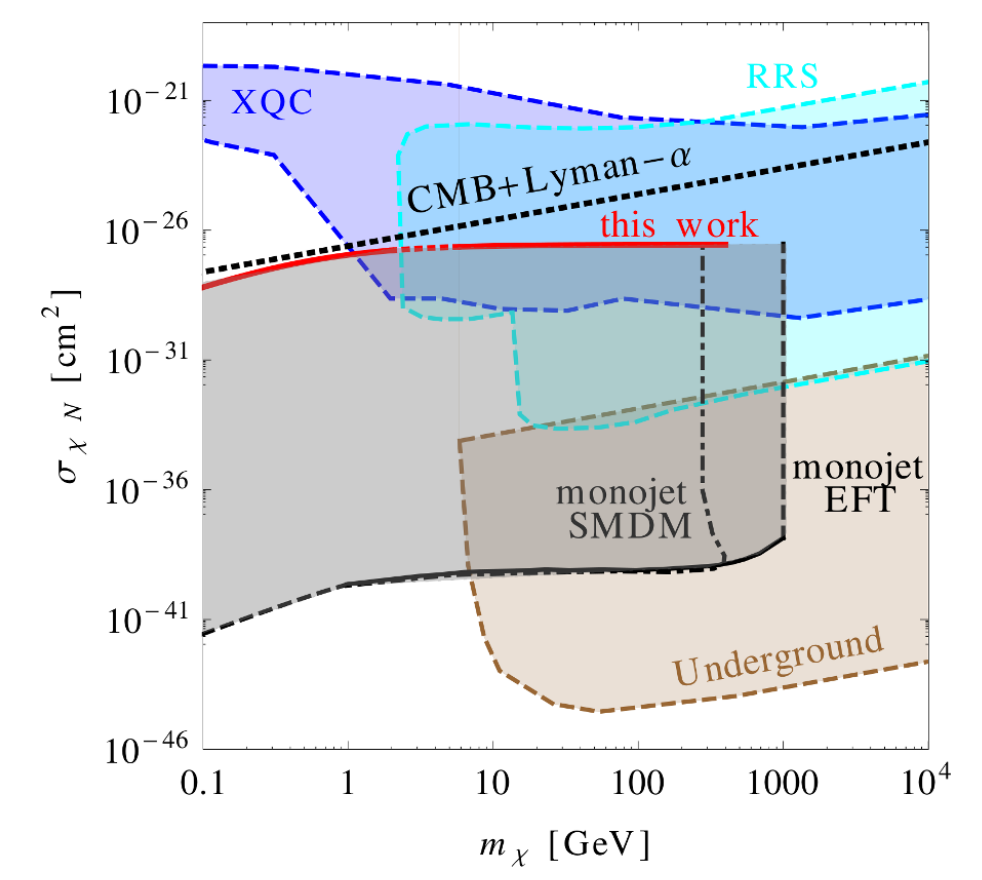
\includegraphics[width=0.8\textwidth]{SIMP_summary.png}\hfill%
  \caption{Summary plot showing the \ac{SIMP} model (red) in comparison with the most important applicable constraints, coming from the LHC monojet analyses (black), the atmospheric XQC and RRS experiments (blue), underground experiments (brown), and the \ac{CMB} observations and Lyman-$\alpha$ data (black dashed line). Figure taken from~\cite{Daci:2015hca}.}
  \label{fig:SIMP_summary}
\end{figure}

\end{itemize}

\clearpage{\pagestyle{empty}\cleardoublepage}
